%% bare_conf_compsoc.tex
%% V1.4b
%% 2015/08/26
%% by Michael Shell
%% See:
%% http://www.michaelshell.org/
%% for current contact information.
%%
%% This is a skeleton file demonstrating the use of IEEEtran.cls
%% (requires IEEEtran.cls version 1.8b or later) with an IEEE Computer
%% Society conference paper.
%%
%% Support sites:
%% http://www.michaelshell.org/tex/ieeetran/
%% http://www.ctan.org/pkg/ieeetran
%% and
%% http://www.ieee.org/

%%*************************************************************************
%% Legal Notice:
%% This code is offered as-is without any warranty either expressed or
%% implied; without even the implied warranty of MERCHANTABILITY or
%% FITNESS FOR A PARTICULAR PURPOSE!
%% User assumes all risk.
%% In no event shall the IEEE or any contributor to this code be liable for
%% any damages or losses, including, but not limited to, incidental,
%% consequential, or any other damages, resulting from the use or misuse
%% of any information contained here.
%%
%% All comments are the opinions of their respective authors and are not
%% necessarily endorsed by the IEEE.
%%
%% This work is distributed under the LaTeX Project Public License (LPPL)
%% ( http://www.latex-project.org/ ) version 1.3, and may be freely used,
%% distributed and modified. A copy of the LPPL, version 1.3, is included
%% in the base LaTeX documentation of all distributions of LaTeX released
%% 2003/12/01 or later.
%% Retain all contribution notices and credits.
%% ** Modified files should be clearly indicated as such, including  **
%% ** renaming them and changing author support contact information. **
%%*************************************************************************


% *** Authors should verify (and, if needed, correct) their LaTeX system  ***
% *** with the testflow diagnostic prior to trusting their LaTeX platform ***
% *** with production work. The IEEE's font choices and paper sizes can   ***
% *** trigger bugs that do not appear when using other class files.       ***                          ***
% The testflow support page is at:
% http://www.michaelshell.org/tex/testflow/



\documentclass[conference,compsoc]{IEEEtran}
% Some/most Computer Society conferences require the compsoc mode option,
% but others may want the standard conference format.
%
% If IEEEtran.cls has not been installed into the LaTeX system files,
% manually specify the path to it like:
% \documentclass[conference,compsoc]{../sty/IEEEtran}

% 직접 추가한 패키지
\usepackage{cleveref, array, booktabs, threeparttable}
\usepackage[labelsep=period, font={footnotesize, sc}]{caption}

\usepackage{tabularx}
\usepackage{graphicx}

\usepackage{kotex}
\usepackage{makecell}

% Some very useful LaTeX packages include:
% (uncomment the ones you want to load)


% *** MISC UTILITY PACKAGES ***
%
%\usepackage{ifpdf}
% Heiko Oberdiek's ifpdf.sty is very useful if you need conditional
% compilation based on whether the output is pdf or dvi.
% usage:
% \ifpdf
%   % pdf code
% \else
%   % dvi code
% \fi
% The latest version of ifpdf.sty can be obtained from:
% http://www.ctan.org/pkg/ifpdf
% Also, note that IEEEtran.cls V1.7 and later provides a builtin
% \ifCLASSINFOpdf conditional that works the same way.
% When switching from latex to pdflatex and vice-versa, the compiler may
% have to be run twice to clear warning/error messages.


% 새롭게 추가한 패키지

% *** CITATION PACKAGES ***
%
\ifCLASSOPTIONcompsoc
  % IEEE Computer Society needs nocompress option
  % requires cite.sty v4.0 or later (November 2003)
  \usepackage[nocompress]{cite}
\else
  % normal IEEE
  \usepackage{cite}
\fi
% cite.sty was written by Donald Arseneau
% V1.6 and later of IEEEtran pre-defines the format of the cite.sty package
% \cite{} output to follow that of the IEEE. Loading the cite package will
% result in citation numbers being automatically sorted and properly
% "compressed/ranged". e.g., [1], [9], [2], [7], [5], [6] without using
% cite.sty will become [1], [2], [5]--[7], [9] using cite.sty. cite.sty's
% \cite will automatically add leading space, if needed. Use cite.sty's
% noadjust option (cite.sty V3.8 and later) if you want to turn this off
% such as if a citation ever needs to be enclosed in parenthesis.
% cite.sty is already installed on most LaTeX systems. Be sure and use
% version 5.0 (2009-03-20) and later if using hyperref.sty.
% The latest version can be obtained at:
% http://www.ctan.org/pkg/cite
% The documentation is contained in the cite.sty file itself.
%
% Note that some packages require special options to format as the Computer
% Society requires. In particular, Computer Society  papers do not use
% compressed citation ranges as is done in typical IEEE papers
% (e.g., [1]-[4]). Instead, they list every citation separately in order
% (e.g., [1], [2], [3], [4]). To get the latter we need to load the cite
% package with the nocompress option which is supported by cite.sty v4.0
% and later.





% *** GRAPHICS RELATED PACKAGES ***
%
\ifCLASSINFOpdf
  % \usepackage[pdftex]{graphicx}
  % declare the path(s) where your graphic files are
  % \graphicspath{{../pdf/}{../jpeg/}}
  % and their extensions so you won't have to specify these with
  % every instance of \includegraphics
  % \DeclareGraphicsExtensions{.pdf,.jpeg,.png}
\else
  % or other class option (dvipsone, dvipdf, if not using dvips). graphicx
  % will default to the driver specified in the system graphics.cfg if no
  % driver is specified.
  % \usepackage[dvips]{graphicx}
  % declare the path(s) where your graphic files are
  % \graphicspath{{../eps/}}
  % and their extensions so you won't have to specify these with
  % every instance of \includegraphics
  % \DeclareGraphicsExtensions{.eps}
\fi
% graphicx was written by David Carlisle and Sebastian Rahtz. It is
% required if you want graphics, photos, etc. graphicx.sty is already
% installed on most LaTeX systems. The latest version and documentation
% can be obtained at:
% http://www.ctan.org/pkg/graphicx
% Another good source of documentation is "Using Imported Graphics in
% LaTeX2e" by Keith Reckdahl which can be found at:
% http://www.ctan.org/pkg/epslatex
%
% latex, and pdflatex in dvi mode, support graphics in encapsulated
% postscript (.eps) format. pdflatex in pdf mode supports graphics
% in .pdf, .jpeg, .png and .mps (metapost) formats. Users should ensure
% that all non-photo figures use a vector format (.eps, .pdf, .mps) and
% not a bitmapped formats (.jpeg, .png). The IEEE frowns on bitmapped formats
% which can result in "jaggedy"/blurry rendering of lines and letters as
% well as large increases in file sizes.
%
% You can find documentation about the pdfTeX application at:
% http://www.tug.org/applications/pdftex





% *** MATH PACKAGES ***
%
%\usepackage{amsmath}
% A popular package from the American Mathematical Society that provides
% many useful and powerful commands for dealing with mathematics.
%
% Note that the amsmath package sets \interdisplaylinepenalty to 10000
% thus preventing page breaks from occurring within multiline equations. Use:
%\interdisplaylinepenalty=2500
% after loading amsmath to restore such page breaks as IEEEtran.cls normally
% does. amsmath.sty is already installed on most LaTeX systems. The latest
% version and documentation can be obtained at:
% http://www.ctan.org/pkg/amsmath





% *** SPECIALIZED LIST PACKAGES ***
%
%\usepackage{algorithmic}
% algorithmic.sty was written by Peter Williams and Rogerio Brito.
% This package provides an algorithmic environment fo describing algorithms.
% You can use the algorithmic environment in-text or within a figure
% environment to provide for a floating algorithm. Do NOT use the algorithm
% floating environment provided by algorithm.sty (by the same authors) or
% algorithm2e.sty (by Christophe Fiorio) as the IEEE does not use dedicated
% algorithm float types and packages that provide these will not provide
% correct IEEE style captions. The latest version and documentation of
% algorithmic.sty can be obtained at:
% http://www.ctan.org/pkg/algorithms
% Also of interest may be the (relatively newer and more customizable)
% algorithmicx.sty package by Szasz Janos:
% http://www.ctan.org/pkg/algorithmicx




% *** ALIGNMENT PACKAGES ***
%
%\usepackage{array}
% Frank Mittelbach's and David Carlisle's array.sty patches and improves
% the standard LaTeX2e array and tabular environments to provide better
% appearance and additional user controls. As the default LaTeX2e table
% generation code is lacking to the point of almost being broken with
% respect to the quality of the end results, all users are strongly
% advised to use an enhanced (at the very least that provided by array.sty)
% set of table tools. array.sty is already installed on most systems. The
% latest version and documentation can be obtained at:
% http://www.ctan.org/pkg/array


% IEEEtran contains the IEEEeqnarray family of commands that can be used to
% generate multiline equations as well as matrices, tables, etc., of high
% quality.




% *** SUBFIGURE PACKAGES ***
%\ifCLASSOPTIONcompsoc
%  \usepackage[caption=false,font=footnotesize,labelfont=sf,textfont=sf]{subfig}
%\else
%  \usepackage[caption=false,font=footnotesize]{subfig}
%\fi
% subfig.sty, written by Steven Douglas Cochran, is the modern replacement
% for subfigure.sty, the latter of which is no longer maintained and is
% incompatible with some LaTeX packages including fixltx2e. However,
% subfig.sty requires and automatically loads Axel Sommerfeldt's caption.sty
% which will override IEEEtran.cls' handling of captions and this will result
% in non-IEEE style figure/table captions. To prevent this problem, be sure
% and invoke subfig.sty's "caption=false" package option (available since
% subfig.sty version 1.3, 2005/06/28) as this is will preserve IEEEtran.cls
% handling of captions.
% Note that the Computer Society format requires a sans serif font rather
% than the serif font used in traditional IEEE formatting and thus the need
% to invoke different subfig.sty package options depending on whether
% compsoc mode has been enabled.
%
% The latest version and documentation of subfig.sty can be obtained at:
% http://www.ctan.org/pkg/subfig

% *** FLOAT PACKAGES ***
%
%\usepackage{fixltx2e}
% fixltx2e, the successor to the earlier fix2col.sty, was written by
% Frank Mittelbach and David Carlisle. This package corrects a few problems
% in the LaTeX2e kernel, the most notable of which is that in current
% LaTeX2e releases, the ordering of single and double column floats is not
% guaranteed to be preserved. Thus, an unpatched LaTeX2e can allow a
% single column figure to be placed prior to an earlier double column
% figure.
% Be aware that LaTeX2e kernels dated 2015 and later have fixltx2e.sty's
% corrections already built into the system in which case a warning will
% be issued if an attempt is made to load fixltx2e.sty as it is no longer
% needed.
% The latest version and documentation can be found at:
% http://www.ctan.org/pkg/fixltx2e


%\usepackage{stfloats}
% stfloats.sty was written by Sigitas Tolusis. This package gives LaTeX2e
% the ability to do double column floats at the bottom of the page as well
% as the top. (e.g., "\begin{figure*}[!b]" is not normally possible in
% LaTeX2e). It also provides a command:
%\fnbelowfloat
% to enable the placement of footnotes below bottom floats (the standard
% LaTeX2e kernel puts them above bottom floats). This is an invasive package
% which rewrites many portions of the LaTeX2e float routines. It may not work
% with other packages that modify the LaTeX2e float routines. The latest
% version and documentation can be obtained at:
% http://www.ctan.org/pkg/stfloats
% Do not use the stfloats baselinefloat ability as the IEEE does not allow
% \baselineskip to stretch. Authors submitting work to the IEEE should note
% that the IEEE rarely uses double column equations and that authors should try
% to avoid such use. Do not be tempted to use the cuted.sty or midfloat.sty
% packages (also by Sigitas Tolusis) as the IEEE does not format its papers in
% such ways.
% Do not attempt to use stfloats with fixltx2e as they are incompatible.
% Instead, use Morten Hogholm'a dblfloatfix which combines the features
% of both fixltx2e and stfloats:
%
% \usepackage{dblfloatfix}
% The latest version can be found at:
% http://www.ctan.org/pkg/dblfloatfix




% *** PDF, URL AND HYPERLINK PACKAGES ***
%
%\usepackage{url}
% url.sty was written by Donald Arseneau. It provides better support for
% handling and breaking URLs. url.sty is already installed on most LaTeX
% systems. The latest version and documentation can be obtained at:
% http://www.ctan.org/pkg/url
% Basically, \url{my_url_here}.




% *** Do not adjust lengths that control margins, column widths, etc. ***
% *** Do not use packages that alter fonts (such as pslatex).         ***
% There should be no need to do such things with IEEEtran.cls V1.6 and later.
% (Unless specifically asked to do so by the journal or conference you plan
% to submit to, of course. )


% correct bad hyphenation here
\hyphenation{op-tical net-works semi-conduc-tor}


\begin{document}
%
% paper title
% Titles are generally capitalized except for words such as a, an, and, as,
% at, but, by, for, in, nor, of, on, or, the, to and up, which are usually
% not capitalized unless they are the first or last word of the title.
% Linebreaks \\ can be used within to get better formatting as desired.
% Do not put math or special symbols in the title.
\title{\LARGE \bf
VISQUIT - Voice IS a Quite Universal Interactive Tool\\
(Kiosk with Vioce Recognition)
}


% author names and affiliations
% use a multiple column layout for up to three different
% affiliations
\author{
\IEEEauthorblockN{Kim Jung Mo}
\IEEEauthorblockA{2014005414\\
Dept. of Information System\\
College of Engineering,\\
Hanyang University\\
Seoul, Rep. of Korea\\
Email: cadenzah93@gmail.com}\\
\IEEEauthorblockN{Lee Ha Min}
\IEEEauthorblockA{2017029134\\
Dept. of Information System\\
College of Engineering,\\
Hanyang University\\
Seoul, Rep. of Korea\\
Email: ggamini7@gmail.com}
\and
\IEEEauthorblockN{Lee Hyo Sik}
\IEEEauthorblockA{2014026208\\
Dept. of Business Management\\
School of Business,\\
Hanyang University\\
Seoul, Rep. of Korea\\
Email: lhslhs9394@gmail.com}\\
\IEEEauthorblockN{Hwang Sung Woo}
\IEEEauthorblockA{2016026599\\
Dept. of Information System\\
College of Engineering,\\
Hanyang University\\
Seoul, Rep. of Korea\\
Email: hsw0194@gmail.com}
}

% conference papers do not typically use \thanks and this command
% is locked out in conference mode. If really needed, such as for
% the acknowledgment of grants, issue a \IEEEoverridecommandlockouts
% after \documentclass

% for over three affiliations, or if they all won't fit within the width
% of the page (and note that there is less available width in this regard for
% compsoc conferences compared to traditional conferences), use this
% alternative format:
%
%\author{\IEEEauthorblockN{Michael Shell\IEEEauthorrefmark{1},
%Homer Simpson\IEEEauthorrefmark{2},
%James Kirk\IEEEauthorrefmark{3},
%Montgomery Scott\IEEEauthorrefmark{3} and
%Eldon Tyrell\IEEEauthorrefmark{4}}
%\IEEEauthorblockA{\IEEEauthorrefmark{1}School of Electrical and Computer Engineering\\
%Georgia Institute of Technology,
%Atlanta, Georgia 30332--0250\\ Email: see http://www.michaelshell.org/contact.html}
%\IEEEauthorblockA{\IEEEauthorrefmark{2}Twentieth Century Fox, Springfield, USA\\
%Email: homer@thesimpsons.com}
%\IEEEauthorblockA{\IEEEauthorrefmark{3}Starfleet Academy, San Francisco, California 96678-2391\\
%Telephone: (800) 555--1212, Fax: (888) 555--1212}
%\IEEEauthorblockA{\IEEEauthorrefmark{4}Tyrell Inc., 123 Replicant Street, Los Angeles, California 90210--4321}}

% use for special paper notices
%\IEEEspecialpapernotice{(Invited Paper)}

% make the title area
\maketitle

% As a general rule, do not put math, special symbols or citations
% in the abstract
\begin{abstract}

VISQUIT is a Kiosk service powered by voice recognition technology based on artificial intelligence. Nowadays, many stores adopt using Kiosk system, by which the cost of hiring clerks and the time spent to make an individual order reduce. The market of Kiosk system is emerging these days, from 60 billion won in 2006 to 250 billion won in 2017. People who are accustomed to digital-based system has no much difficulty using this type of new method in store, but for those people who are digitally illiterate, even ordering their meal in a restaurant is a hard task. To solve the problem with current Kiosk system's poor user experience, we suggest using voice recognition technology to compose the ordering system's UI. This can effectively replace the previous "select-based" ordering system with "speech-based". Also, our sevice will help expanding the Kiosk's market size by providing better machine with better user experience and reasonable price to customers and restaurant owners. Based on this approach, we will develop and propose new paradigm of designing UI of Kiosk system.

\end{abstract}

% no keywords




% For peer review papers, you can put extra information on the cover
% page as needed:
% \ifCLASSOPTIONpeerreview
% \begin{center} \bfseries EDICS Category: 3-BBND \end{center}
% \fi
%
% For peerreview papers, this IEEEtran command inserts a page break and
% creates the second title. It will be ignored for other modes.
\IEEEpeerreviewmaketitle

\section{Introduction}

\subsection{Motivation}
Kiosks are unmanned machine that can take orders on behalf of a clerk. Recently, the installation and operation of kiosks is increasing, especially in franchise restaurants. This saves labor costs for the personnel required to place an order and allows more orders to be processed in unit time.

However, some people suffer from the appearance of kiosks. That people are who are not familiar with these Digital technology.  In particular, for older people, they are very new to digital technology. According to the National Information Society Agency (NIA) '2018 Digital Information Gap Survey,' the overall 'digital information level' for the elderly aged 55 or older is only 63.1\% of the general public. The contrary situation arises where the marginalized class exists due to the emergence of technology to make people convenient.
% 조사한 자료는 인용으로 바꾸자

\subsection{Problem Analysis}
Among the problems of kiosks, we will focus on improving the ordering / payment software installed inside the kiosks. In the conventional method, as all the menus are displayed on the screen, the amount of information increases, which causes inconvenience to those who are not familiar with the UI. In addition, in order to maximize the amount of information displayed, the size of text and images is small, and the screen resolution is limited, so the display is not clear. In addition, the sensitivity of the touch screen is not as accurate as that of the physical buttons, providing a confusing UX to the user.

\subsection{Solution}
Using the artificial intelligence speech recognition technology of SKTelecom's NUGU Platform, the user's speech is recognized and ordered based on it. This provides a familiar interface to users who are not familiar with digital technology, as if they are talking to a real person. It can also handle multiple orders without the need for a complex UI.

In addition, the UI is configured to maximize the clarity of the content by using a large image and text, and to better understand the content by users with low vision. As the size of the content increases, the amount of information that can be contained on one screen decreases, so the UI is designed to implement the same business logic as the existing despite the reduced amount of information.

According to Auction catalog, the price range of Kiosk machines purchased in the market is various, but it costs at least 1 million won, which can reach up to 10 million won. This is not an affordable cost for small businesses. Also, purchasing Kiosk machine and reducing clerks will not result immediate cost savings, so restaurant owners will hesitate to purchase the machine. SKTelecom's NUGU speaker costs 79,000 won, which is maximum 90\% cheaper than previous Kiosk machine, so it will not be a too much burden for small businesses.

\section{Requirements}

\subsection{User side (Store Customer)}

\subsubsection{View Menu List (ID 101)}
\begin{enumerate}
  \item Provide menu list with paper or tablet
\end{enumerate}

\subsubsection{Order by Voice (ID 102)}
\begin{enumerate}
  \item SKT NUGU Speaker handles this
  \item Accept orders according to Intent and Entity
  % \item Intent (order.burger, order.set, order.side, order.beverage, order.morning, etc) 
  % \item Entity (Burgers, sets, sides, beverages, mornings, BID_QT_COUNT, etc) 
\end{enumerate}

\subsubsection{Check Menu (ID 103)}
\begin{enumerate}
  \item Send an order from the Nugu speaker to the backend proxy
  \item Process total orders in Backend proxy based on Entity
  \item Transfer the aggregated order back to the Nugu speaker to confirm the order using the TTS function
  \item Send user confirmation to backend proxy
\end{enumerate}

\subsubsection{Payment (ID 104)}
\begin{enumerate}
  \item Customer could pay with card  
\end{enumerate}

\subsection{Client Side (Store Owner)}

\subsubsection{Log-in (ID 201)}
\begin{enumerate}
  \item To identify clients, require client to log in  
\end{enumerate}

\subsubsection{Menu update (ID 202)}
\begin{enumerate}
  \item Client could add new menu
  \item Client could delete menu
  \item Client could modify menu  
\end{enumerate}

\subsubsection{View Order History (ID 203)}
\begin{enumerate}
  \item Client could see order lists customers ordered
  \item Client could see order history already served
\end{enumerate}


\subsection{Server Side}

\subsubsection{Check order (ID 301)}
\begin{enumerate}
  \item Sum menu input from NUGU
  \item Response to NUGU
  \begin{enumerate}
    \item Receive orders from the Nugu speaker with Intent and Entity and send them to server
    \item Aggregate orders based on Entity in the Backend proxy
    \item Send aggregated orders on the Nugu speakers
    \item Order confirmed by user with TTS function in NUGU speaker
    \item If the order is correct, backend proxy stores the order in DB
  \end{enumerate}
\end{enumerate}

\subsubsection{Send order to database (ID 302)}
\begin{enumerate}
  \item Server get orders from NUGU speaker
  \item Server keep these orders in database  
\end{enumerate}


\subsubsection{Make json for NUGU (ID 303)}
\begin{enumerate}
  \item Server should make json file for learning of NUGU speaker  
\end{enumerate}


\section{Development Environment}

\subsection{Software Development Platforms}

We chose Web environment to develop our project. Many applications can be run on the Web. Web technology(Node.js) will be used to show that voice kiosks work properly. In addition, we will use AWS commercial cloud platforms such as EC2, S3, RDS etc. to apply what we have learned in class. Lastly, SKT's NUGU API will be used to analyze users' voice commands and translate them into text.

\subsubsection{Node.js}

Node.js is an open-source, cross-platform, JavaScript runtime environment that executes JavaScript code outside of a browser. Node.js lets developers use JavaScript to write command line tools and for server-side scripting—running scripts server-side to produce dynamic web page content before the page is sent to the user's web browser. Consequently, Node.js represents a "JavaScript everywhere" paradigm, unifying web application development around a single programming language, rather than different languages for server- and client-side scripts.

\subsubsection{React.js}

React (also known as React.js or ReactJS) is a JavaScript library for building user interfaces. It is maintained by Facebook and a community of individual developers and companies. React can be used as a base in the development of single-page or mobile applications, as it is optimal for fetching rapidly changing data that needs to be recorded.

\subsubsection{Amazon Web Service EC2}

Configure an environment where applications can be developed and distributed quickly without the need for physical hardware equipment. Deploy as many virtual servers as you want, configure your security, network, and manage your storage. A sudden change in resources configured for the service can quickly scale up or down depending on the changes, reducing the need for forecasting server traffic.

\subsubsection{Amazon Web Service S3}

Amazon S3 or Amazon Simple Storage Service is a service offered by Amazon Web Services (AWS) that provides object storage through a web service interface. Amazon S3 uses the same scalable storage infrastructure that Amazon.com uses to run its global e-commerce network. Amazon S3 can be employed to store any type of object which allows for uses like storage for Internet applications, backup and recovery, disaster recovery, data archives, data lakes for analytics, and hybrid cloud storage. In its service-level agreement, Amazon S3 guarantees 99.9\% uptime, which works out to less than 43 minutes of downtime per month.

\subsubsection{Amazon Web Service RDS}

Amazon Relational Database Service (or Amazon RDS) is a distributed relational database service by Amazon Web Services (AWS). It is a web service running "in the cloud" designed to simplify the setup, operation, and scaling of a relational database for use in applications. Administration processes like patching the database software, backing up databases and enabling point-in-time recovery are managed automatically. Scaling storage and compute resources can be performed by a single API call as AWS does not offer an ssh connection to RDS instances.

\subsubsection{SKTelecom NUGU API}

Based on SK Telecom's technical skills such as voice recognition, voice synthesis, and understanding of natural language through NUGU developers, the company can develop new functions and provide NUGU's various functions through voice command in devices or applications owned by its affiliates. We will recognize and categorize the user's voice commands through the NUGU API and send output results to the user via voice.

\subsubsection{Docker}

Docker is a set of platform-as-a-service (PaaS) products that use OS-level virtualization to deliver software in packages called containers. Containers are isolated from one another and bundle their own software, libraries and configuration files; they can communicate with each other through well-defined channels. All containers are run by a single operating-system kernel and are thus more lightweight than virtual machines. The service has both free and premium tiers. The software that hosts the containers is called Docker Engine. It was first started in 2013 and is developed by Docker, Inc. 

\subsection{Programming Languages}

\subsubsection{Javascript}

Javascript is a high-level, interpreted scripting language that conforms to the ECMAScript specification. Javascript has flexible grammars: freedom from indentation, loose type checks. Also, it adopts modern progamming padigms and has convenient and great features: function programming, reactive programming. By using this language we can learn various modern progamming paradigms. Javascript is used in web browsers, which means it does not require any special working environment to run program written by Javascript.

\subsection{Cost Estimation}

This project heavily rely on Amazon Web Service. The cost estimation is in Table 1. This is calculated by Amazon Web Service Cost Calulator.

\begin{table}[ht!] \renewcommand\arraystretch{1.25}
  \begin{threeparttable}
      \caption{Role assignment for each participants of this project%
      \label{tab:table1}}    %% Caption above tabular, label inside caption
      \begin{tabular}{@{}l l>{\raggedright\arraybackslash}p{3.8cm}@{}}
      \toprule
      \bfseries Service & \bfseries Region & \multicolumn{1}{l}{\bfseries Cost(Monthly)} \\
      \midrule
      Amazon EC2 & Asia Pacific (Seoul) & USD(\$) 11.65 \\
      Amazon RDS & Asia Pacific (Seoul) & USD(\$) 19.64 \\
      \bottomrule
      \end{tabular}
  \end{threeparttable}
\end{table}

\subsection{Development Environment Description}

Used development environment tools information is described in Table 2.

\begin{table}[ht!] \renewcommand\arraystretch{1.25}
  \begin{threeparttable}
      \caption{Role assignment for each participants of this project%
      \label{tab:table2}}    %% Caption above tabular, label inside caption
      \begin{tabular}{@{}l l>{\raggedright\arraybackslash}p{3.8cm}@{}}
      \toprule
      \bfseries Name & \bfseries Version & \multicolumn{1}{l}{\bfseries Description} \\
      \midrule
      Windows & 10 Pro & Operating System made by Microsoft \\
      macOS & Catalina(10.15) & Operating System made by Apple, used in Macbook \\
      Ubuntu & 16.04.6 & Operating System developed by Linux Foundation \\
      Visual Studio Code & 1.39.1 & Text editor and Integrated Development Editor made by Microsoft \\
      Atom.io & 1.40.1 & Text editor and Integrated Development Editor made by GitHub \\
      iTerm2 & 3.3.6 & Terminal Emulator used in macOS \\
      Z shell(zsh) & 5.7.1 & Unix shell for CLI \\
      \bottomrule
      \end{tabular}
  \end{threeparttable}
\end{table}

\subsection{Market Research \& Software in Use}
% Software in Use

\subsubsection{Kiosk Market in Korea}
Unmanned stores are spreading all over the world. The unmanned store are actively being made due to artificial intelligence, the Internet of Things, the development of sensor technology, the lack of labor force and the minimum wage hike. South Korea has been burdened with labor costs following a 10-percent minimum wage hike for two consecutive years, and the unmanned era is in full swing due to the spread of an "untact" culture that is reluctant to contact. In restaurants, customers order on their own through KIOSK. And unmanned convenience stores have begun to sprout up everywhere. As of 2017, the size of South Korea's kiosk market is estimated to be around 250 billion won, with a high annual growth rate of 14 percent. The market, which stood at only 60 billion won in 2006, rose to 180 billion won in 2013 and rose to 250 billion won in 2017.

\subsubsection{Voice Recognition ARS}
The ARS allowed us to perform the tasks we needed without waiting time. However, the initial ARS was a one-sided way of listening and pressing buttons. As people got used to ARS services, they started feeling that services provided by the ARS is not enough. In addition, people used only limited number of services. Considering these factors, ARS through voice recognition will be able to provide services only requested by users. By doing this, services can be provided much more effectively, by which the time and cost for developing unnecessary features.

\subsubsection{Voice Recognition AI}
There are services in the market called artificial intelligence voice assistant such as Bixby, Siri, Nugu and Gigagenie. Despite providing convenient services, many people are reluctant to use these services. Understanding these reasons will be helpful for us to envision the services we will provide in the future.

\subsubsection{Delivery Application}
We think the delivery app is in the same situation as the kiosk we are currently thinking about. Orders, which were previously made through voice-to-speech conversations over the phone, have been made possible through the application with several touch points. There are many advantages, such as the availability of personalized orders through delivery apps, but it is still a far from those who are not familiar with digital culture. If Kiosk's problem is solved, it is believed that the delivery app will be able to solve the problem in the same way later.

\subsubsection{Starbucks Siren Order with Voice}
T-Map x NUGU introduced a voice service for Starbucks' "Siren Order". The combination of "T-Map x Nugu" and "Siren Order" makes it possible for users to order for various Starbucks products with voice, even while driving. Orders are based on voice while driving, followed by beverage selection, neighborhood store selection, order product confirmation, order receipt and payment. In addition, by linking to T-map's functionalities, the app will forward the order to the store when it is expected to arrive the store within 5 minutes. As a result, the user experience will be improved as waiting time for the ordered beverages will decrease and the freshness of the product will be maintained.

\subsection{Task Distribution}

Task Distribution is shown in Table 3. Note that each project participants periodically switched their roles with the others to apply different perspectives and improve their expriences.

\begin{table}[ht!] \renewcommand\arraystretch{1.25}
  \begin{threeparttable}
      \caption{Task distribution  for each participants of this project%
      \label{tab:table1}}    %% Caption above tabular, label inside caption
      \begin{tabular}{@{}l l>{\raggedright\arraybackslash}p{4.7cm}@{}}
      \toprule
      \bfseries Task & \bfseries Assignee & \multicolumn{1}{l}{\bfseries Description} \\
      \midrule
      Project Manager & Lee Hyo Sik & Schedule overall development plan and assign proper jobs to team members \\ 
      Consumer & Kim Jung Mo & Test and try out a prototype application, gather the potential improvement \\ 
      User & Lee Ha Min & Gather basic feature requirement for this project by asking questionnaires the elderly near the university. \\ 
      Developer & Hwang Sung Woo & Prepare a development environment for this project and build up the application \\
      \bottomrule
      \end{tabular}
  \end{threeparttable}
\end{table}

\section{Specification}

\subsection{User side}

\subsubsection{View Menu List (ID 101)}
\begin{enumerate}
  \item Client should provide menu  
\end{enumerate}

\subsubsection{Order by Voice (ID 102)}
\begin{enumerate}
  \item Quantity of a menu in a order cannot pass 10
  \item End ordering when customers say '주문 끝'  
\end{enumerate}


\subsubsection{Check Menu (ID 103)}
\begin{enumerate}
  \item NUGU speaker asks customers whether order is right  
\end{enumerate}


\subsection{Client Side}

\subsubsection{Log-in (ID 201)}
\begin{enumerate}
  \begin{figure}[ht!]
    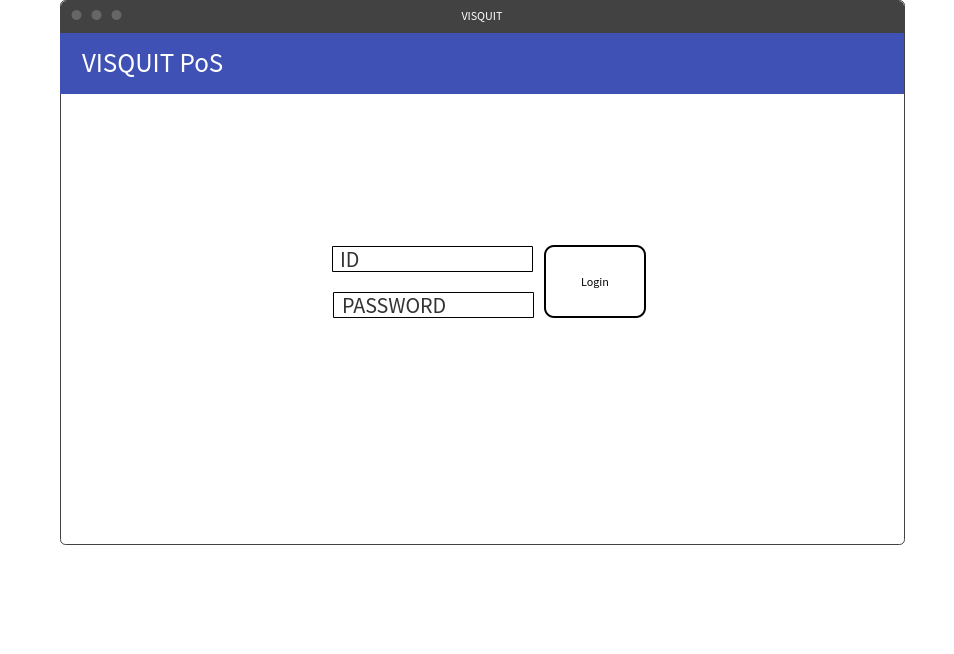
\includegraphics[width=\linewidth]{figures/mockup/Login.png}
    \caption{Login}
    \label{fig:mockup}
  \end{figure}  
  \item Client could login with SKT ID  
  \begin{figure}[ht!]
    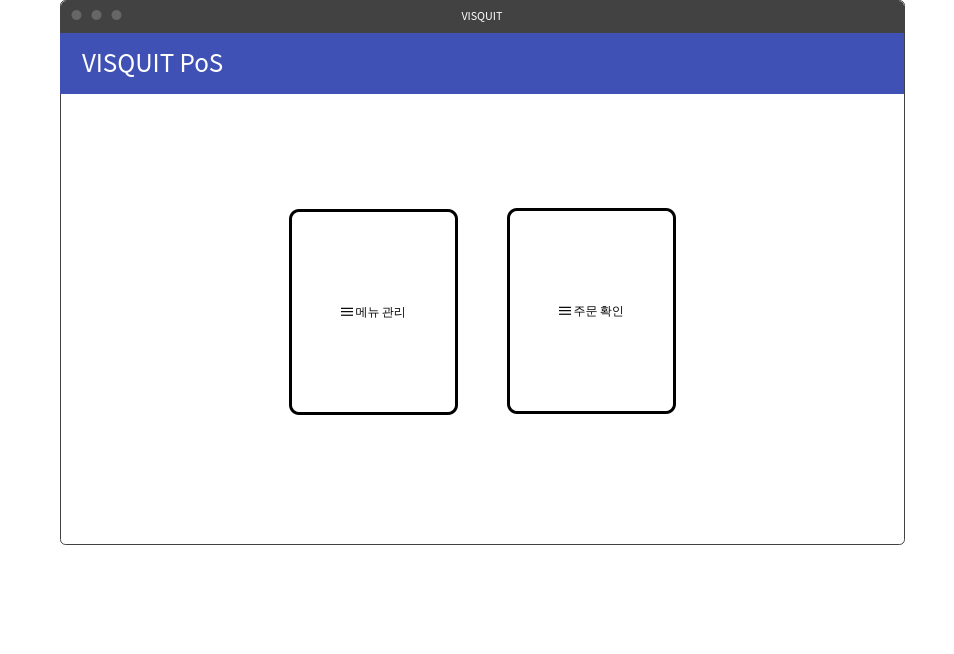
\includegraphics[width=\linewidth]{figures/mockup/Main.png}
    \caption{Main}
    \label{fig:mockup}
  \end{figure}
  \item After log-in clients could choose menu management or check order list
\end{enumerate}


\subsubsection{Menu update (ID 202)}
\begin{enumerate}
  \begin{figure}[ht!]
    \includegraphics[width=\linewidth]{figures/mockup/Menu_list.png}
    \caption{Menu management}
    \label{fig:mockup}
  \end{figure}
  \item Client could see menu list of the store
  \begin{figure}[ht!]
    \includegraphics[width=\linewidth]{figures/mockup/Add_menu.png}
    \caption{Add Menu}
    \label{fig:mockup}
  \end{figure}
  \item Clients should enter menu name and price to add menu
  \item Clients should check all the synonyms for learning of NUGU speaker
\end{enumerate}


\subsubsection{View Order History (ID 203)}
\begin{enumerate}
  \begin{figure}[ht!]
    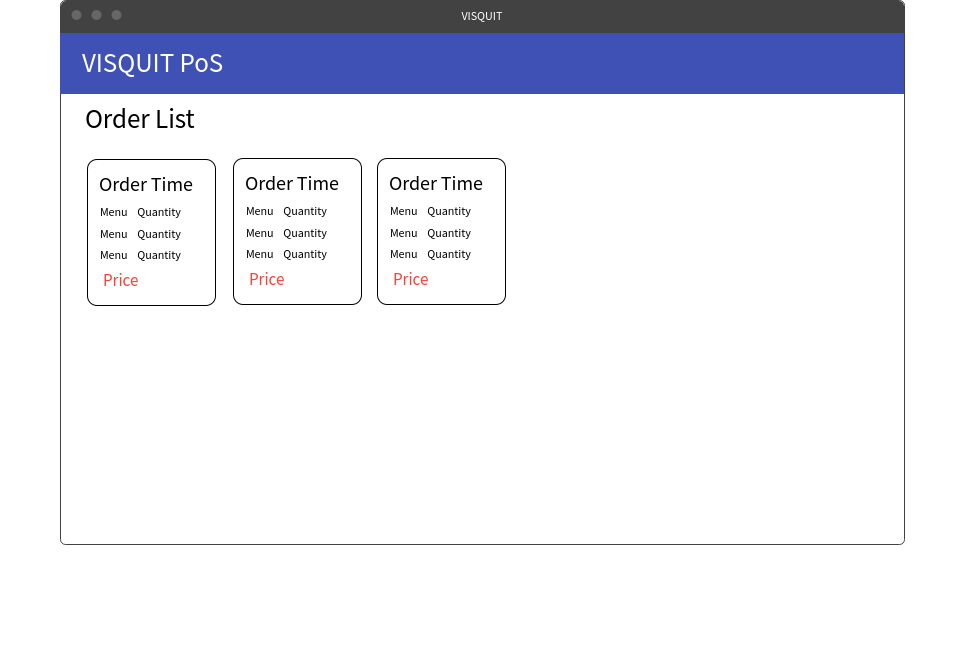
\includegraphics[width=\linewidth]{figures/mockup/OrderList.png}
    \caption{Order List}
    \label{fig:mockup}
  \end{figure}
  \item Clients could see order lists in a page
  \begin{figure}[ht!]
    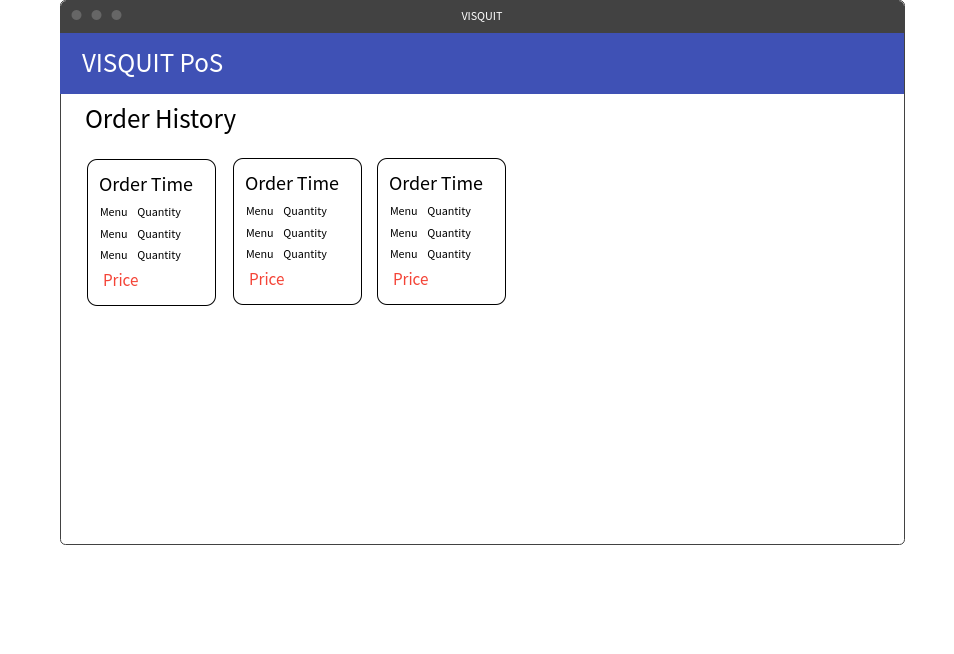
\includegraphics[width=\linewidth]{figures/mockup/OrderHistory.png}
    \caption{Order History}
    \label{fig:mockup}
  \end{figure}
  \item When orders are served client could see orders in order history
\end{enumerate}


\subsection{Server Side}

\subsubsection{Check order (ID 301)}
\begin{enumerate}
  \item When customer order, NUGU speaker check each menus
  \item Customer should confirm what they ordered
  \item Server give customers order number
  \item Customer can check what they ordered with order number  
\end{enumerate}

\subsubsection{Send order to database (ID 302)}
\begin{enumerate}
  \item When customer confirm all the orders, server confirm the orders and keep in database  
\end{enumerate}

\subsubsection{Make json for NUGU (ID 303)}
\begin{enumerate}
  \item When clients update menu, server should make json file
\end{enumerate}


\section{Architecture Design}

\subsection{Overall Architecture}

Our service is web-based application and heavily depends on Amazon Web Service for deployment. Our application's UI is implemented with React.js. Our server is implemented by Node.js with Express.js web server on it to serve service data to frontend UI as REST API, and interact with SKTelecom NUGU's API and speaker. Entire API server is running on Amazon Web Service EC2 instance, where Nginx L4 switch stands in front of dockerized Node.js Web Application Servers. Figure 1 shows overall architecture of the service.

\begin{figure}[ht!]
  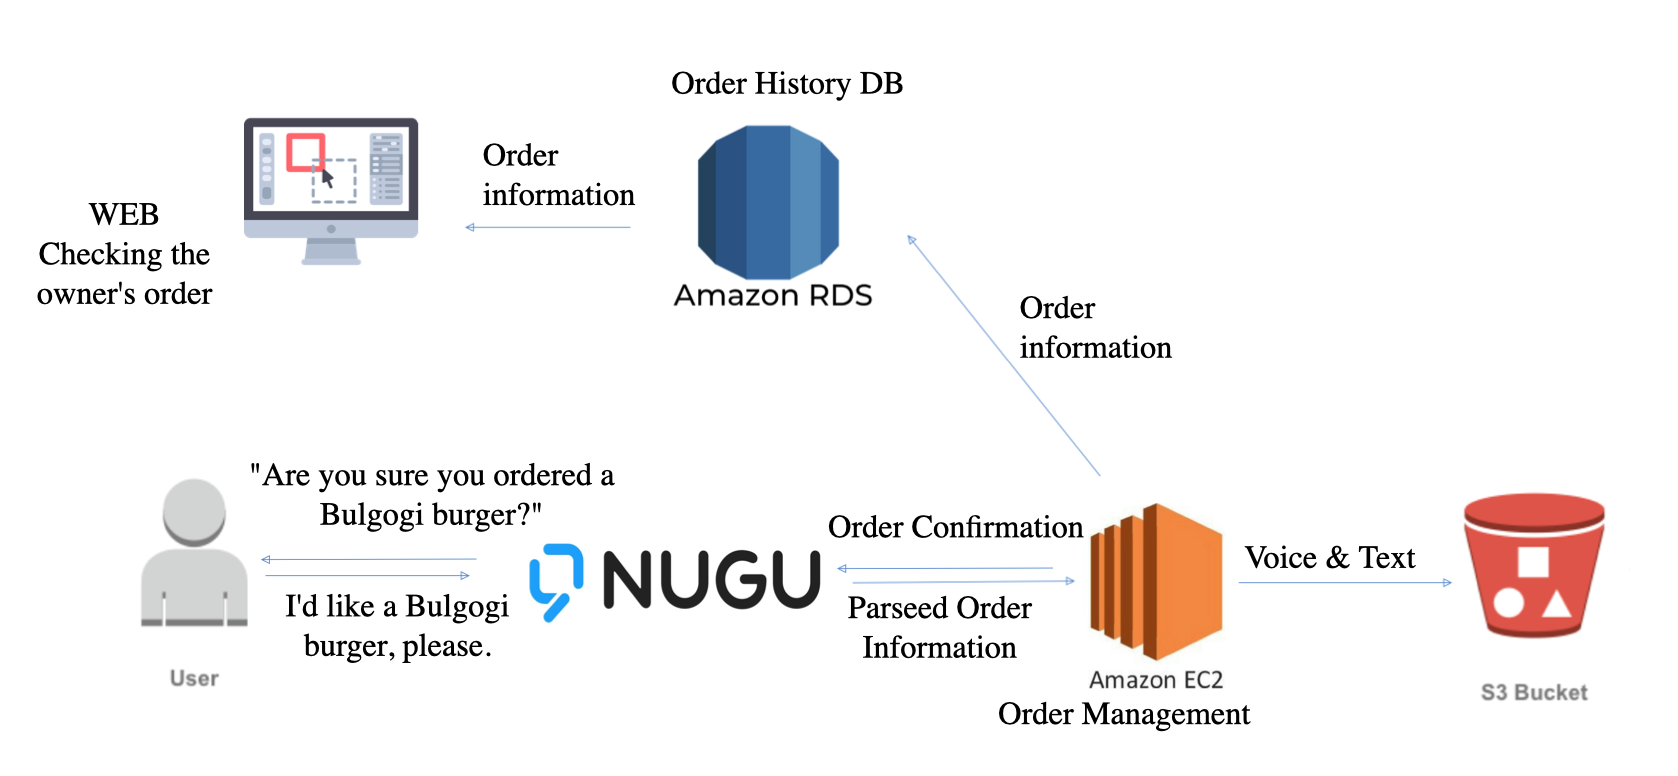
\includegraphics[width=\linewidth]{figures/architecture.png}
  \caption{Overall system architecture diagram}
  \label{fig:architecture}
\end{figure}

\subsection{NUGU Architecture Design}
Below are in-voice commands required to make interaction with SKTelecom NUGU Speaker.  

\subsubsection{General Setting}
\begin{itemize}
  \item Backend Proxy Server:
  \item Web URL: TBA
  \item Exception message : “Err Code 404 서버에 연결하지 못했습니다”
\end{itemize}

\subsubsection{Intent}
\begin{enumerate}
  \item Welcome.with.NUGU.INTENT.open
  \begin{itemize}
    \item Precondition : In case play session entry is the Innovation Name NUGU.For INTENT.open (In case “Start/Open” is mentioned with the Invocation name)
    \item Does this INTENT need backend proxy? YES
    \item Output : 안녕하세요 비스킷입니다. 무엇을 주문하시겠어요? 메뉴 하나씩 주문해주세요.
  \end{itemize}
  
  \item Order
  \begin{enumerate}
    \item Order request
    \begin{itemize}
      \item Command : (menu), (count), (ending of word) ex) 불고기와퍼 한 개 줘
      \begin{table}[h!] \renewcommand\arraystretch{1.75}
      \centering
      \begin{tabular}{@{}c | c c c@{}}
      \hline
      Example mention & 불고기 와퍼 & 한 개  & 줘               \\ 
      \hline
      Category        & menu   & count & ending of word  \\ 
      \hline
      Entity          & MENU   & COUNT & STATEMENT       \\
      \hline
      \end{tabular}
      \end{table}      
    \end{itemize}
    
    \item request sample
    CODE
    
    \item Does this INTENT need backend proxy? YES
    
    \item Action for Order Intent : order\_confirm
    \begin{table}[h!] \renewcommand\arraystretch{1.25}
      \centering
        \begin{tabular}{@{}c | c c c c@{}}
        \hline
        \makecell{NUGU \\ response} & 불고기 와퍼 & 한 개 & 주문되었습니다 & \makecell{더 주문할 것 \\ 있으신가요?}  \\ 
        \hline
        Category        & menu   & count & mention & mention \\ 
        \hline
        \makecell{Utterance \\ parameter}  & menu & count & fixed statement & fixed statement \\
        \hline
        \end{tabular}
    \end{table}  
  
  \end{enumerate}

  \item Ask something
  \begin{enumerate}
    \item ask.taste
    \begin{itemize}
      \item ask some menu is salty or not.
      \item Command : (menu), (ending of word) ex) 불고기와퍼 싱거워?
      \begin{table}[h!] \renewcommand\arraystretch{1.75}
        \centering
          \begin{tabular}{@{}c | c c @{}}
          \hline
          Example mention & 불고기 와퍼 & 싱거워?  \\ 
          \hline
          Category        & menu   & ending of word  \\ 
          \hline
          Entity  & MENU   & TASTE   \\
          \hline
          \end{tabular}
      \end{table}  

      \item Does this INTENT need backend proxy? NO
      \item Action for ask.taste : answer\_taste
      \begin{table}[h!] \renewcommand\arraystretch{1.75}
        \centering
          \begin{tabular}{@{}c | c c c @{}}
          \hline
          NUGU response & 불고기 와퍼 & 는  & 짠편입니다 \\ 
          \hline
          Category        & menu   & postposition & taste \\ 
          \hline
          Utterance parameter  & {{menu}}   & fixed postposition & {{taste}} \\
          \hline
          \end{tabular}
      \end{table}  
    \end{itemize}
    
    \item ask.spicy
    \begin{itemize}
      \item ask some menu is spicy of not.
      \item Command : (menu), (ending of word) ex) 불고기와퍼 매워?
      \begin{table}[h!] \renewcommand\arraystretch{1.75}
        \centering
          \begin{tabular}{@{}c | c c @{}}
          \hline
          Example mention & 불고기 와퍼 & 매워?  \\ 
          \hline
          Category        & menu   & ending of word  \\ 
          \hline
          Entity  & MENU   & SPICY   \\
          \hline
          \end{tabular}
      \end{table}  

      \item Does this INTENT need backend proxy? NO
      \item Action for ask.spicy : answer\_spicy
      \begin{table}[h!] \renewcommand\arraystretch{1.75}
        \centering
          \begin{tabular}{@{}c | c c c @{}}
          \hline
          NUGU response & 불고기 와퍼 & 는  & 맵지않습니다 \\ 
          \hline
          Category        & menu   & postposition & spicy \\ 
          \hline
          Utterance parameter  & {{menu}}   & fixed postposition & {{spicy}} \\
          \hline
          \end{tabular}
      \end{table} 
      
    \end{itemize}

    \item ask.recommend
    \begin{itemize}
      \item ask to recommend delicious menu.
    \end{itemize}
  \end{enumerate}

  \item End\_Order
  \begin{enumerate}
    \item Say you don’t have anything to order
    \item Command : (menu), (ending of word) ex) 불고기와퍼 매워? 
    \begin{table}[h!] \renewcommand\arraystretch{1.25}
      \centering
        \begin{tabular}{@{}c | c  @{}}
        \hline
        Example mention & 더 주문할거 없어 \\ 
        \hline
        Category        & tell no more order \\ 
        \hline
        Entity  & END \\
        \hline
        \end{tabular}
    \end{table} 

    \item request sample
    CODE
    \item Does this INTENT need backend proxy? YES
    \item Action for End\_Order : End\_Order
    \begin{table}[h!] \renewcommand\arraystretch{1.25}
      \centering
        \begin{tabular}{@{}c | c c @{}}
        \hline
        NUGU response & 주문이 완료되었습니다 \\ 
        \hline
        Category        & statement \\ 
        \hline
        Utterance parameter  & fixed statement \\
        \hline
        \end{tabular}
    \end{table} 

  \end{enumerate}

  \item Check ordered Menu
\end{enumerate}

\subsubsection{Entitiy}
\begin{enumerate}
  \item Menu
  \begin{itemize}
    \item Menus to order
    \begin{table}[h!] \renewcommand\arraystretch{1.25}
      \centering
        \begin{tabular}{@{}c | c @{}}
        \hline
        Parameter & synonym \\ 
        \hline
        불고기와퍼 & \makecell{불고기와퍼, 와퍼불고기, \\ 불고기 들어간 와퍼} \\ 
        \hline
        치즈와퍼 & \makecell{치즈와퍼, 와퍼치즈, \\ 치즈 들어간 와퍼, \\ 치즈맛 와퍼} \\
        \hline
        치즈스틱 & 치즈스틱, 스틱치즈 \\
        \hline
        콜라 & 콜라, coke \\
        \hline
        아이스아메리카노 &	\makecell{아이스아메리카노, \\ 아메리카노 아이스, \\ 시원한 아메리카노} \\
        \hline
        따뜻한아메리카노	& \makecell{따뜻한아메리카노, \\ 아메리카노 따뜻한거, \\ 아메리카노 핫} \\
        \hline
        \end{tabular}
    \end{table} 

  \end{itemize}

  \item COUNT
  \begin{itemize}
    \item Quantity of menu
    \begin{table}[h!] \renewcommand\arraystretch{1.25}
      \centering
        \begin{tabular}{@{}c | c @{}}
        \hline
        Parameter & synonym \\ 
        \hline
        1 & 한개, 하나, 한잔, 하나만 \\ 
        \hline
        2 & 두개, 두잔 \\
        \hline
        3 & 세개, 세잔 \\
        \hline
        ... & ... \\
        \hline
        \end{tabular}
    \end{table} 

  \end{itemize}

  \item END
  \begin{itemize}
    \item Indicate the termination of order.
    \begin{table}[h!] \renewcommand\arraystretch{1.25}
      \centering
        \begin{tabular}{@{}c | c @{}}
        \hline
        Parameter & synonym \\ 
        \hline
        END & \makecell{END, 더 없어, \\ 주문끝, 없어, \\ 없습니다, …}	 \\ 
        \hline
        \end{tabular}
    \end{table} 

  \end{itemize}

  \item Statement
  \begin{itemize}
    \item Conjunctive Ending
    \begin{table}[h!] \renewcommand\arraystretch{1.25}
      \centering
        \begin{tabular}{@{}c | c @{}}
        \hline
        Parameter & synonym \\ 
        \hline
        주세요 & 줘, 요, 주세요, 줘요	 \\ 
        \hline
        \end{tabular}
    \end{table} 

  \end{itemize}
\end{enumerate}

\subsubsection{Actions}
\begin{enumerate}
  \item NUGU.ACTION.Welcome
  \begin{itemize}
    \item Action when first entering a play
    \item Play call name (Invocation name) and NUGU, as shown in ‘아리야 VISQUIT 시작’ in Device Standby (IDLE).When igniting INTENT.open together, - In this case, the Prompt corresponding to ‘Invocation name only’ will be mentioned, after which Prompt will be switched on, and the Prompt will be referred to as ‘Standby Prompt’.
    \item This action is taken when the user enters the play by mentioning the name of the play and the Custom Intent inside the play, such as ‘아리야 VISQUIT에서 아이스아메리카노 한잔 줘’ in the Device Standby (IDLE). - In this case, the Prompt corresponding to the ‘Invocation name and Intent’ are glued to the front of the response These are called ‘continuous Prompt’.
  \end{itemize}
  
  \item NUGU.ACTION.exit
  \begin{itemize}
    \item NUGU, where the user is in the Play session, including ‘주문 종료’ and ‘더 주문할거 없어’.Operation is performed when INTENT.stop is in placed.
    \item After Prompt has been triggered, the session ends and returns to the IDLE state. These Prompts are referred to as ‘End Prompt’.
  \end{itemize}

  \item NUGU.ACTION.rewind
  \begin{itemize}
    \item NUGU, for example, user ‘다시’.Action in case of ignition corresponding to INTENT.rewind.
    \item This action does not have a response and performs a command to play the most recent response from scratch.
  \end{itemize}

  \item NUGU.ACTION.fallback
  \begin{itemize}
    \item Action triggered in case of not being able to handle this play
    \item This will work if the user has made a mention within the Play session but does not have the Intent to process.
    \item Action that works when the user says ‘다시’
    \item A situation with no Intent to process, i.e. a Fallback situation, is a complex type that mixes the end type and the standby type to form Prompt.
  \end{itemize}

  \item Order\_confirm
  \begin{itemize}
    \item Confirm the order to the customer and send the order to the server
  \end{itemize}

  \item End\_order
  \begin{itemize}
    \item A function that terminates an order.
    \item When this function is enabled, it informs the server that the order has been terminated.
  \end{itemize}

  \item Check\_order
  \begin{itemize}
    \item Request when you want to check the customer’s order
    \item Invoke orders from the database and forward them through the server to the NUGU speaker to speak to the customer.
  \end{itemize}

\end{enumerate}

\subsection{Database Design}

\begin{figure}[ht!]
  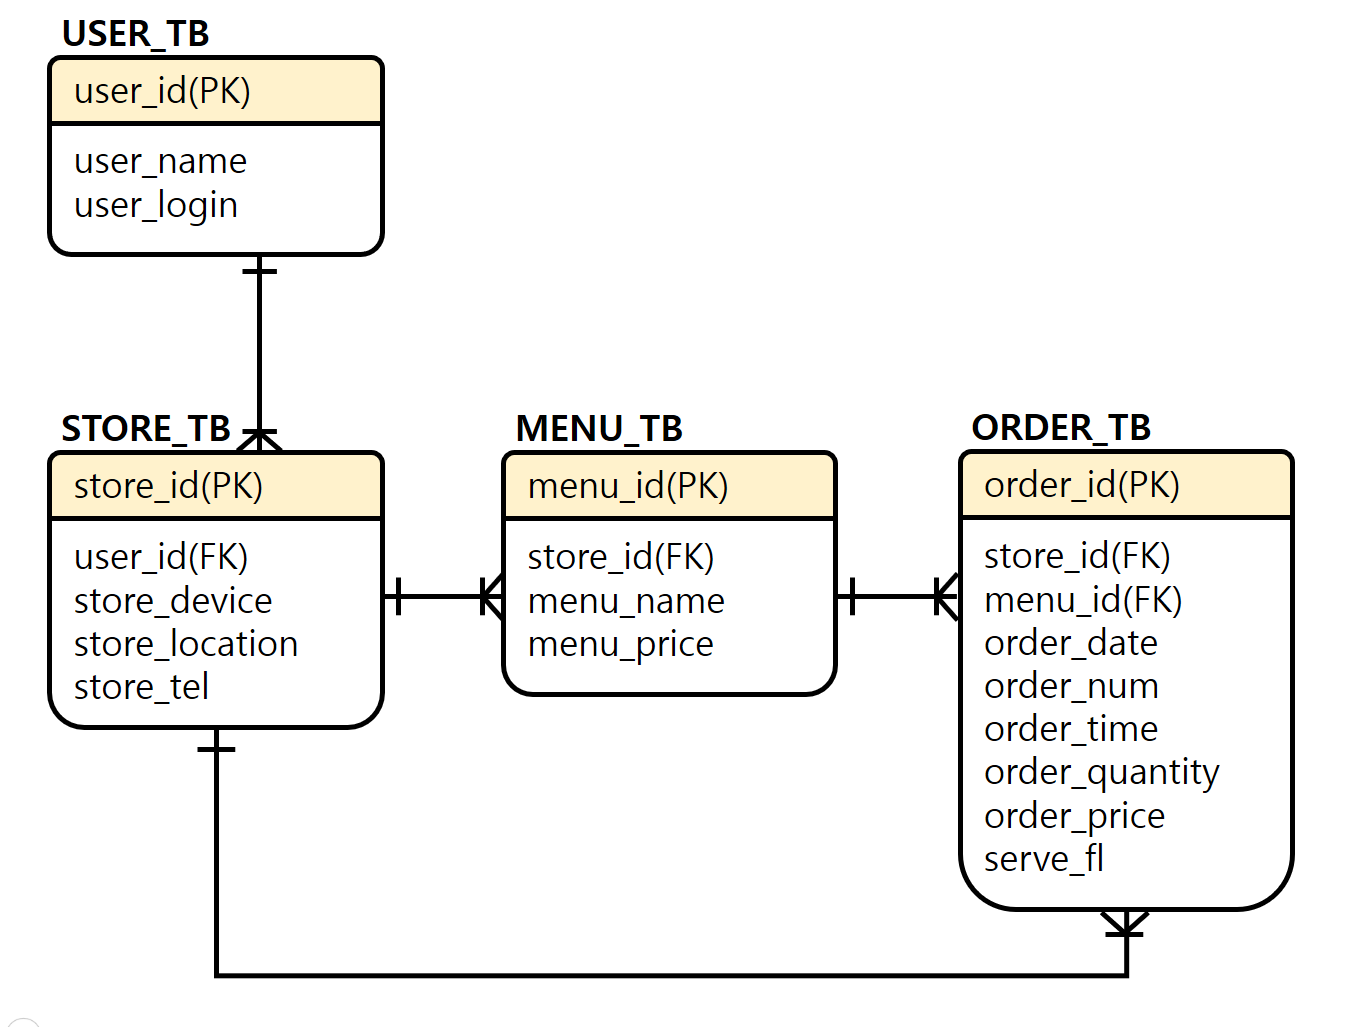
\includegraphics[width=\linewidth]{figures/database.PNG}
  \caption{Database architecture diagram}
  \label{fig:database}
\end{figure}

\subsubsection{USER\_TB}
\begin{itemize}
  \item user\_id(PK): identification of user(store owner)
  \item user\_name: user's name
  \item user\_login: information of user login(like token)
\end{itemize}

\subsubsection{STORE\_TB}
\begin{itemize}
  \item store\_id(PK): identification of store
  \item user\_id(FK): reference USER\_TB table
  \begin{itemize}
    \item one user could own multiple shops
  \end{itemize}
  \item store\_device: NUGU speaker device identification of each store
  \item store\_location: location information of the store
  \item store\_tel: telephone number of the store
\end{itemize}

\subsubsection{MENU\_TB}
\begin{itemize}
  \item menu\_id(PK): identification of menu
  \item store\_id(FK): reference STORE\_TB table
  \begin{itemize}
    \item one store could have multiple menus
  \end{itemize}
  \item menu\_name: name of menu
  \item menu\_price: price of menu
\end{itemize}

\subsubsection{ORDERS\_TB}
\begin{itemize}
  \item order\_id(PK): identification of order
  \item store\_id(FK): reference STORE\_TB table
  \item menu\_id(FK): reference MENU\_TB table
  \begin{itemize}
    \item one menu could be ordered multiple times
  \end{itemize}
  \item order\_date: date of order
  \item order\_num: number of order
  \item order\_time: time information of the order
  \item order\_quantity: quantity of menu in order
  \item order\_price: price of menu\_id times order\_quantity
  \item serve\_fl: flag of information whether order is served or not
\end{itemize}


\subsection{Directory Organization - Frontend}

Table 4 shows the directory organization of React.js frontend application's project.

\begin{table}[ht!] \renewcommand\arraystretch{1.25}
  \begin{threeparttable}
      \caption{Directory Organization for Frontend Application Project%
      \label{tab:table5}}    %% Caption above tabular, label inside caption
      \begin{tabular}{@{}l l>{\raggedright\arraybackslash}p{3.2cm}@{}}
      \toprule
      \bfseries Directory & \bfseries File name(s) & \multicolumn{1}{l}{\bfseries Modules used} \\
      \midrule
      /src/components & Component.js & Storybook \\
      /src/containers & ComponentContainer.js & Redux.js, axios \\
      /src/pages & App.js, Page.js & React Router \\
      /redux & module.js & Redux.js \\
      .storybook & config.js, addon.js & Storybook \\
      \bottomrule
      \end{tabular}
  \end{threeparttable}
\end{table}

\subsubsection{/components}
React codes implementing each UI assets used to compose the Frontend UI. Basic design concept is based on Material-UI and we modified it according to our purpose.

\subsubsection{/containers}
React codes including states, event listeners, and functions used in each pages. The structure and workflow are based on Redux. States and functions are initialized in this code and passed into each UI components.

\subsubsection{/pages}
Index codes where each routings start. Each routings are provided via React Router. Our service's frontend UI is rendered by React-based client-side rendering, where page routing executes in frontend, not backend.

\subsubsection{.storybook}
Storybook is a test framework that eases developers by allowing to check each design assets independently on the screen rapidly. With storybook, we can check if a design asset is correctly implemented without running entire service, improving efficiency of development process and easing the communication with designers and planners.

\subsubsection{Axios}
Axios is Promise based HTTP client for the browser and Node.js. It is used to request data from API server.

\subsubsection{Webpack}
Webpack is a module bundler used to combine all codes and resources in a project into a single file, also providing size minifying. Our service is optimized with Webpack to rapidly serve our web page to users.

\subsubsection{Babel}
Babel is a JavaScript transpiler that converts React syntax into plain JavaScript codes, downgrades ES6+ JavaScript syntax into ES5 syntax. This is a required module to execute React-based project.


\subsection{Directory Organization - Backend}
\begin{table}[ht!] \renewcommand\arraystretch{1.25}
  \begin{threeparttable}
    \caption{Directory Organization for Backend Application Project%
    \label{tab:table6}}    %% Caption above tabular, label inside caption
    \begin{tabular}{@{}l l>{\raggedright\arraybackslash}p{3.2cm}@{}}
    \toprule
    \bfseries Directory & \bfseries File name(s) & \multicolumn{1}{l}{\bfseries Modules used} \\
    \midrule
      /api/store &	index.js, store.controller.js	& Express, Sequelize \\
      /api/menu &	index.js, menu.controller.js	& Express, Sequelize \\
      /api/common & baseResult.js, & - \\
      /config & sequelize.json & - \\
      /models & MENU-TB.js & Sequelize \\
      /bin	& www.js	& Express \\
      .	& app.js, Dockerfile	& Express \\
      \bottomrule
      \end{tabular}
  \end{threeparttable}
\end{table}

\subsubsection{/api/store}
Node.js codes implementing API that related to store information and 'make order' business logic. In API, Express and Sequelize modules are used.

\subsubsection{/api/menu} 
Node.js codes implementing API that related to menu-information business logic. In API, Express and Sequelize modules are used.

\subsubsection{/api/common} 
Node.js codes including basic API response format, function that checks whether HTTP Request sender is legit or not and event-handler on some specific HTTP connection event. 

\subsubsection{/config}
In order to use sequelize module in Node.js file, configuration about DB connection needed. sequelize.json files contain database name,address of host ,password and type of database.

\subsubsection{/models}
Querying database using sequelize needs certain model definition or configuration about table in that database. In models folders, all table in database are defined in JavaScript syntax. Then Index.js file imports that *table-definition JavaScript file* and sets connection between Node.js and Sequelize module.

\subsubsection{/bin}
Entry point of visquit-backend service. In www.js file, using express module,listen specific port.

\subsubsection{app.js,Dockerfile}
app.js routes incoming HTTP request into proper API handler. We use Docker , so docker configuration file,Dockerfile,needed.

\subsubsection{Express}
Express is Web framework used in our project. Using this module, we don't *reinvent the wheel* about HTTP service. Express provide simple and convenient middle-ware like routing,error-handler,cookie and parser. Many of above middle-ware can be implemented custom way that we want to make.

\subsubsection{Sequelize}
We use ORM(Object-relational mapping) module named Sequelize for database querying. Using this module, we don't have to write *long and complex* SQL Query statement, just simply use function like findOne,findAll,destroy,create to get data from database.

\subsubsection{express-list-endpoints} 
Simple module that list all API entry point URL and type(GET,POST,PUT,PATCH,DELETE) . We use this module to print out currently implemented API list. 

\subsubsection{bodyParser} 
In order to parsing HTTP request body, we use bodyParser module.

\section{Use Cases}

\subsection{Frontend UI}

\subsubsection{Initial Landing}

\begin{figure}[ht!]
  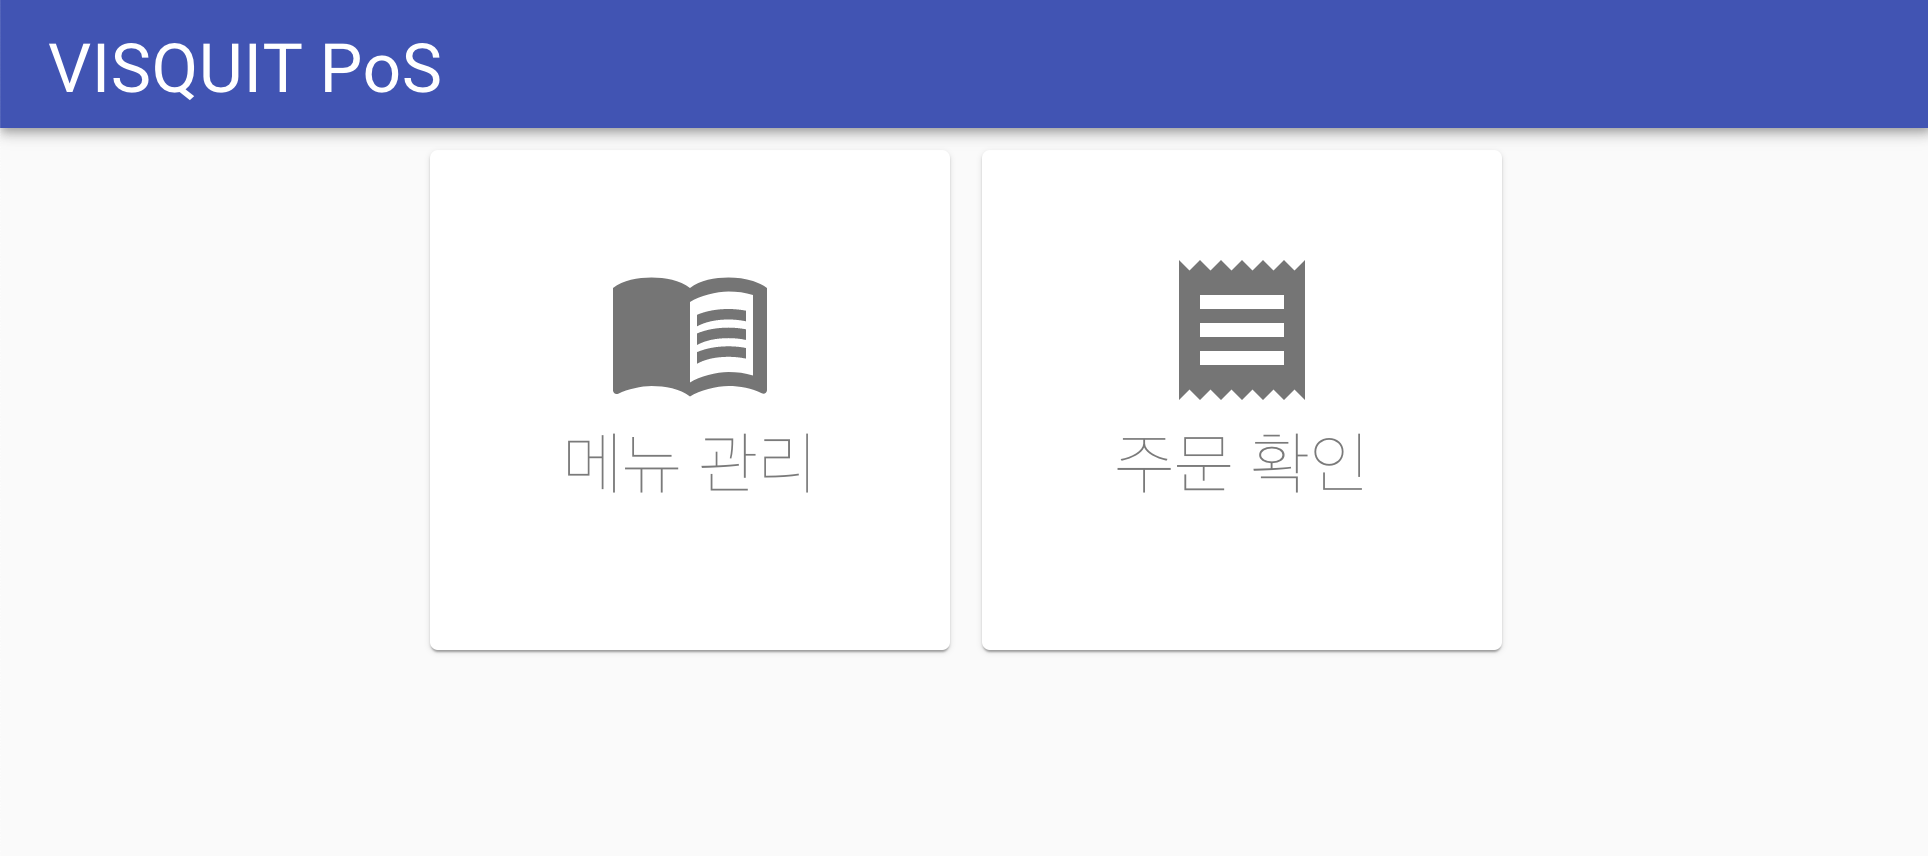
\includegraphics[width=\linewidth]{figures/frontend/01-landing.png}
  \caption{Initial Landing Page of Frontend UI}
  \label{fig:01-landing}
\end{figure}

When a user (typically, a restaurant's owner or manager) access our service, he or she will see this initial landing page. Then the user can choose which feature to use.

\subsubsection{View Menu List}

\begin{figure}[ht!]
  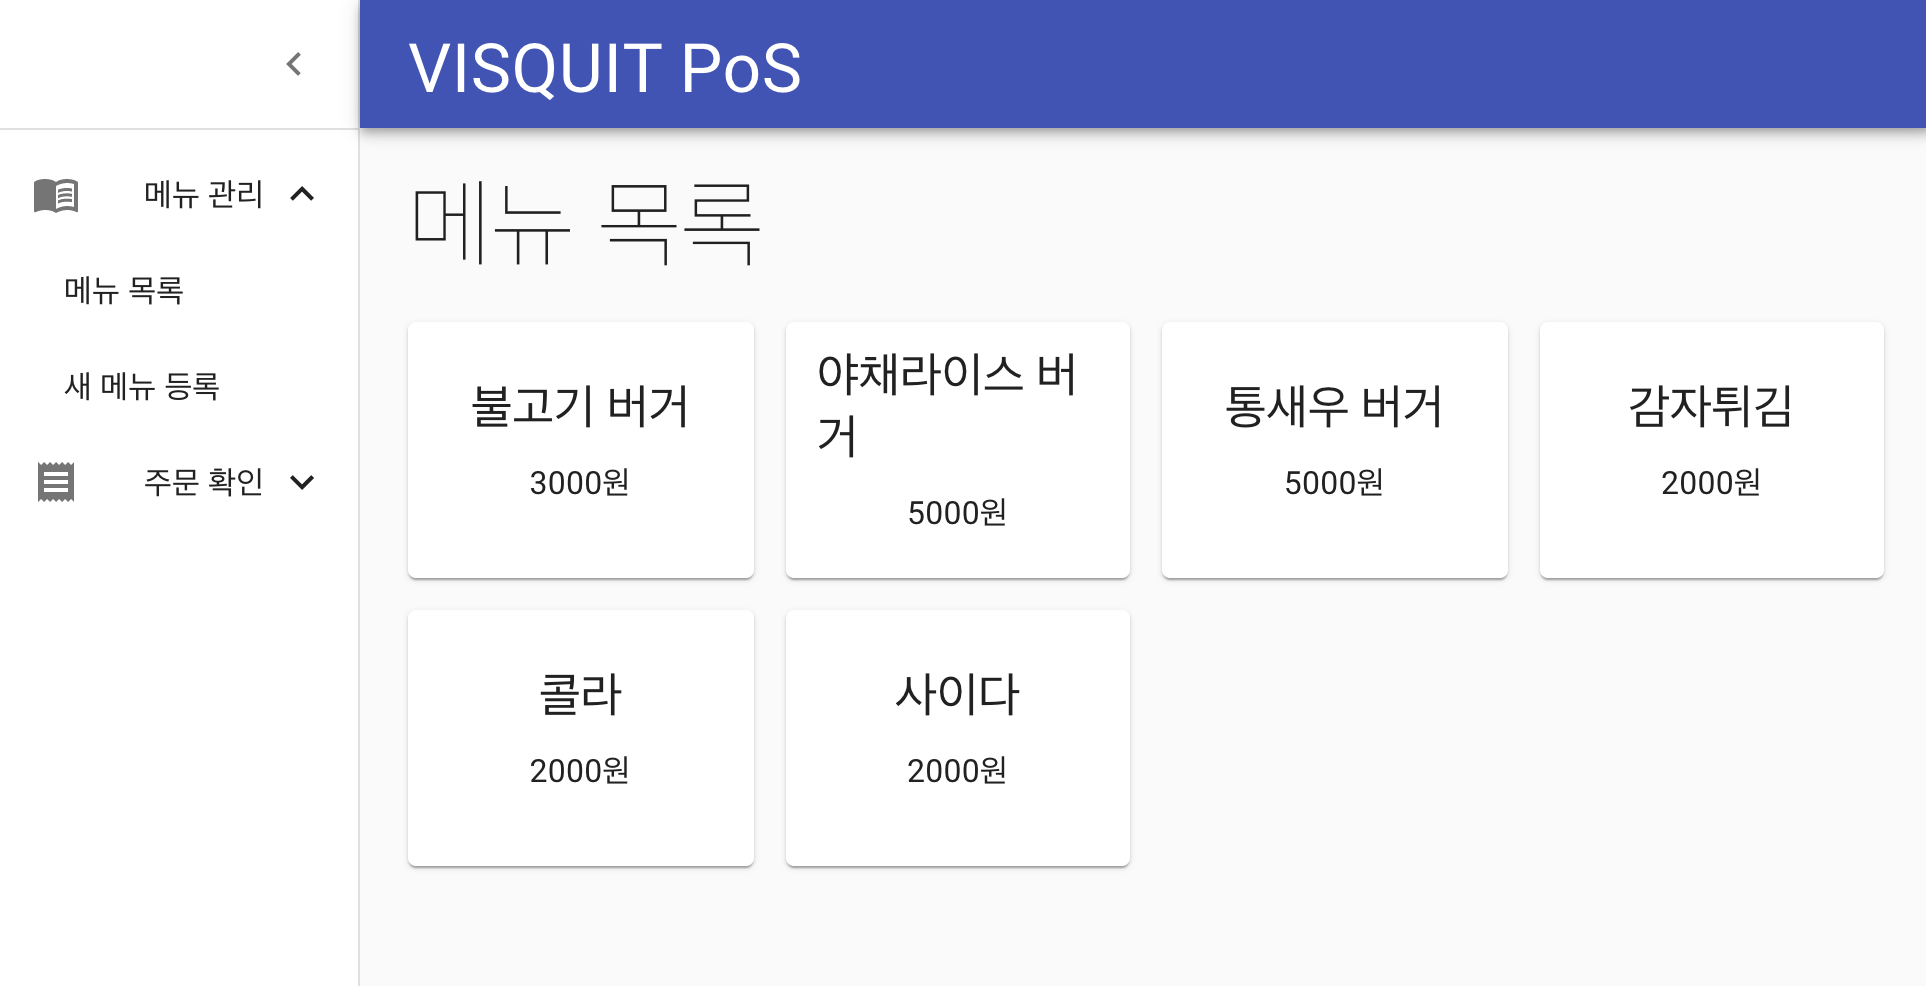
\includegraphics[width=\linewidth]{figures/frontend/02-menulist.png}
  \caption{Viewing menu list}
  \label{fig:02-menulist}
\end{figure}

The user can view all menus registered in the user's context, where only menus served at the user's restaurant are shown. If the user click the arrow button on top-left side, the menu bar can be toggled to hide or be shown.

\subsubsection{Add New Menu}

\begin{figure}[ht!]
  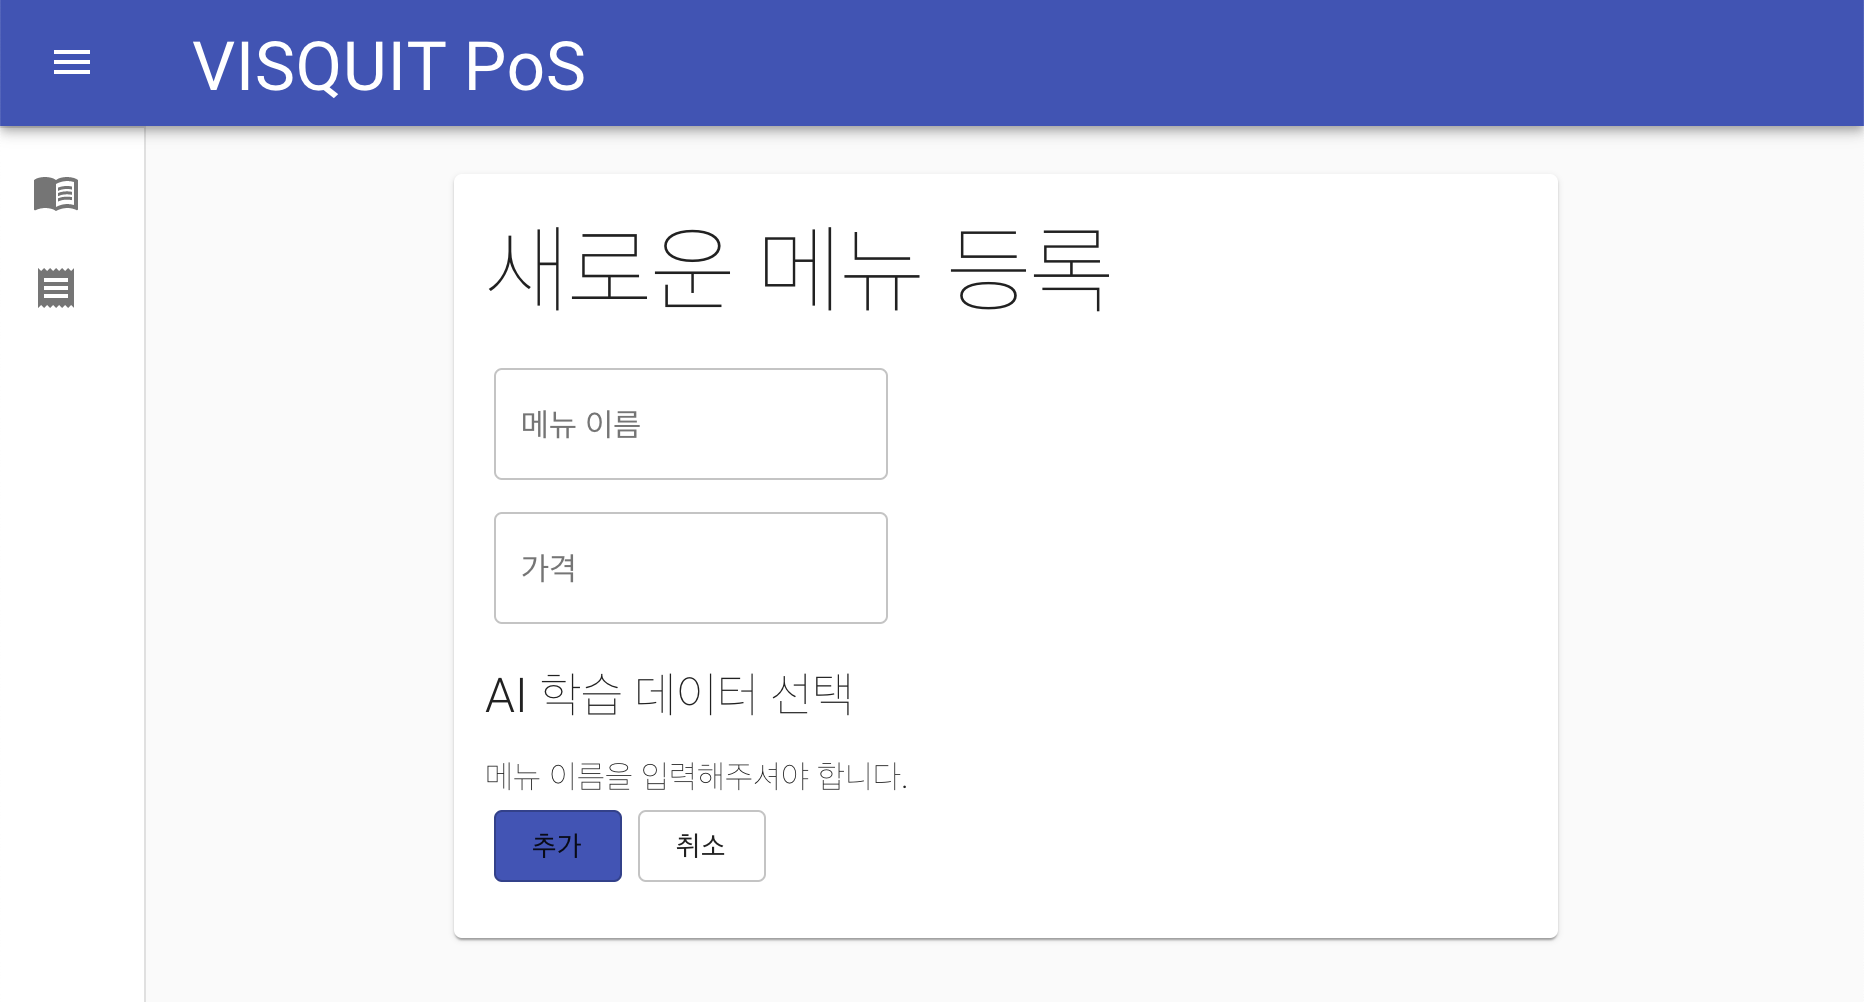
\includegraphics[width=\linewidth]{figures/frontend/03-newmenu-landing.png}
  \caption{Page of Adding New Menu}
  \label{fig:03-newmenu-landing}
\end{figure}

When clicking '새 메뉴 등록' the button on the left, the user will be routed to menu adding page. The user can fill each forms and these values will be sent to the server.

\subsubsection{Generating String Data for AI's Learning}

\begin{figure}[ht!]
  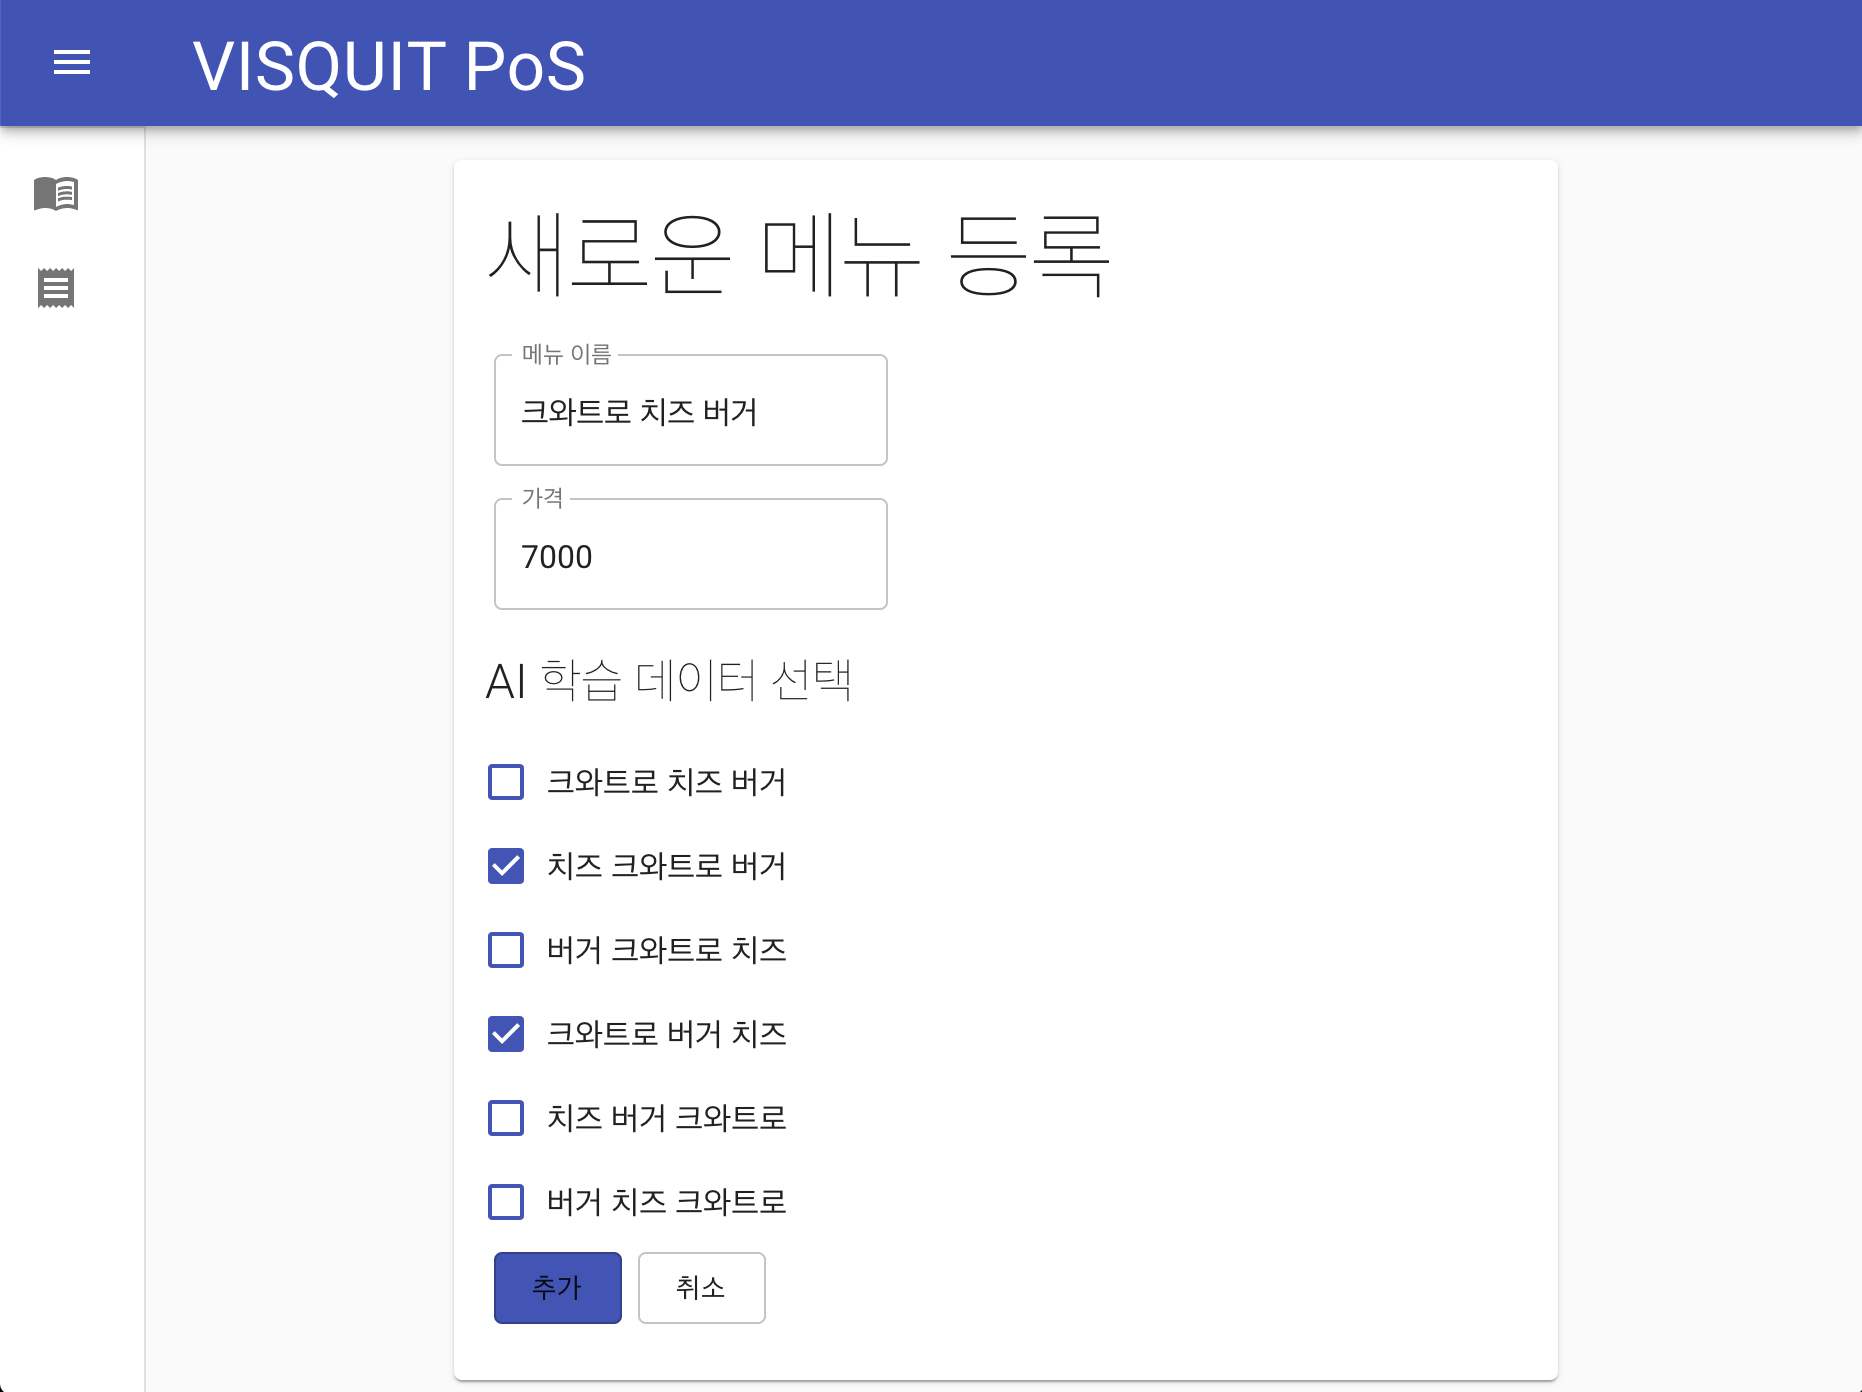
\includegraphics[width=\linewidth]{figures/frontend/04-newmenu-ai.png}
  \caption{Generating String data for AI's Learning}
  \label{fig:04-newmenu-ai}
\end{figure}

For SKTelecom's NUGU Speaker's AI to construct model for processing menu data, it is helpful to provide learning data of a new menu from frontend logic. When the user types in a new menu's name, that string will be used for generating all possible permutations of menu names. For example, if the user types in '콰트로 치즈 버거', then the frontend logic will autometically generate '콰트로 치즈 버거', '치즈 콰트로 버거', '콰트로 버거 치즈', ... etc. After that, the user can choose what to pass to the server for learning.

\subsubsection{Prompting Modal for each actions}

\begin{figure}[ht!]
  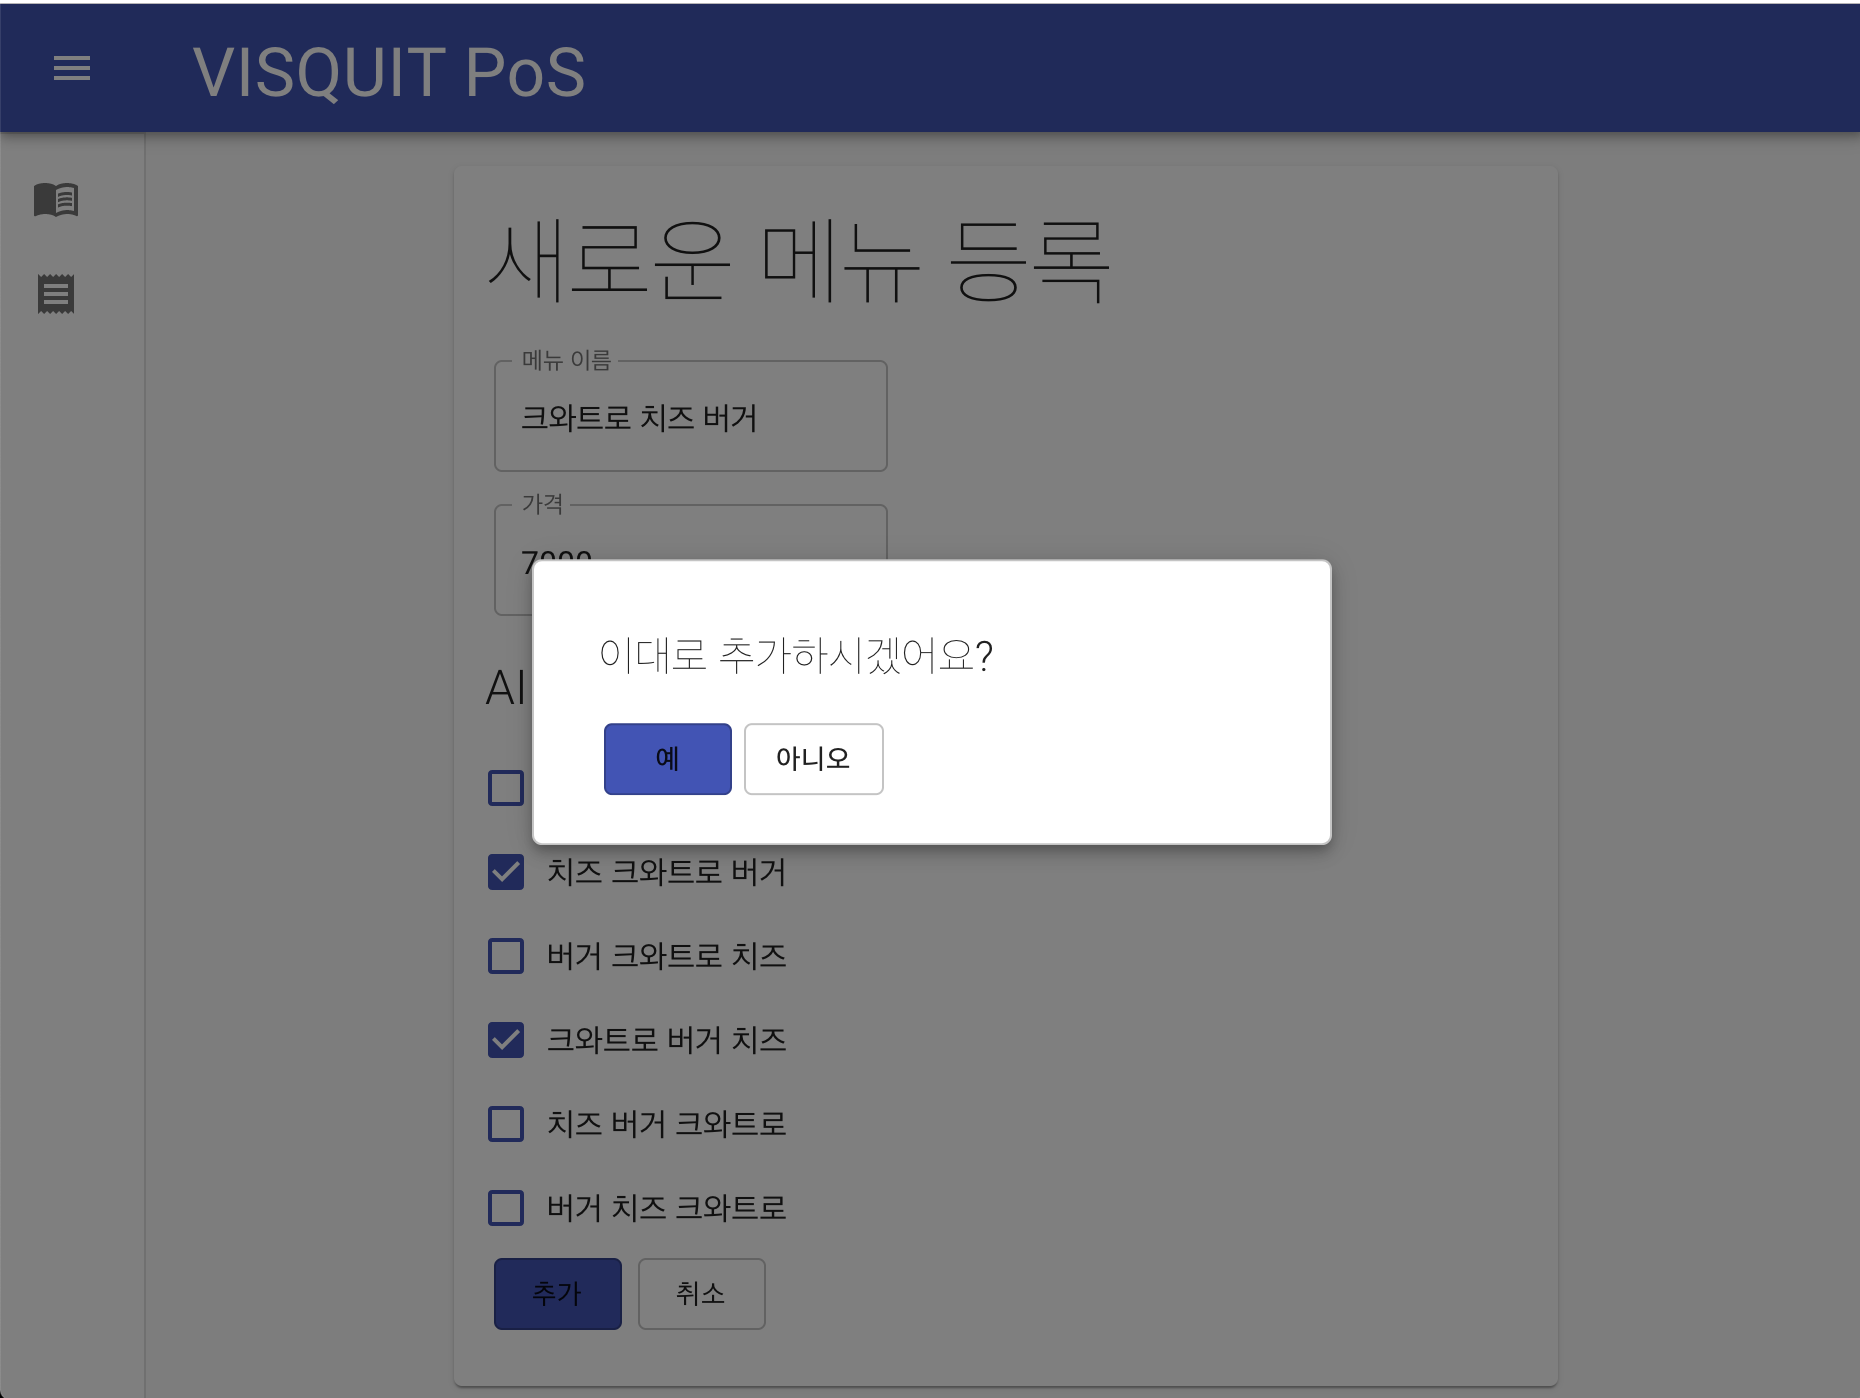
\includegraphics[width=\linewidth]{figures/frontend/05-newmenu-modal.png}
  \caption{Prompting Modal for each actions}
  \label{fig:05-newmenu-modal}
\end{figure}

The user's each actions that triggers interaction with REST API will be double-checked by frontend UI. If the user tries to create, update, or delete a menu, a modal window will be shown on the top of the UI and ask again. When the user clicks '예', the intended action will be executed. Else, the action will be aborted.

\subsubsection{Edit Previous Menu}

\begin{figure}[ht!]
  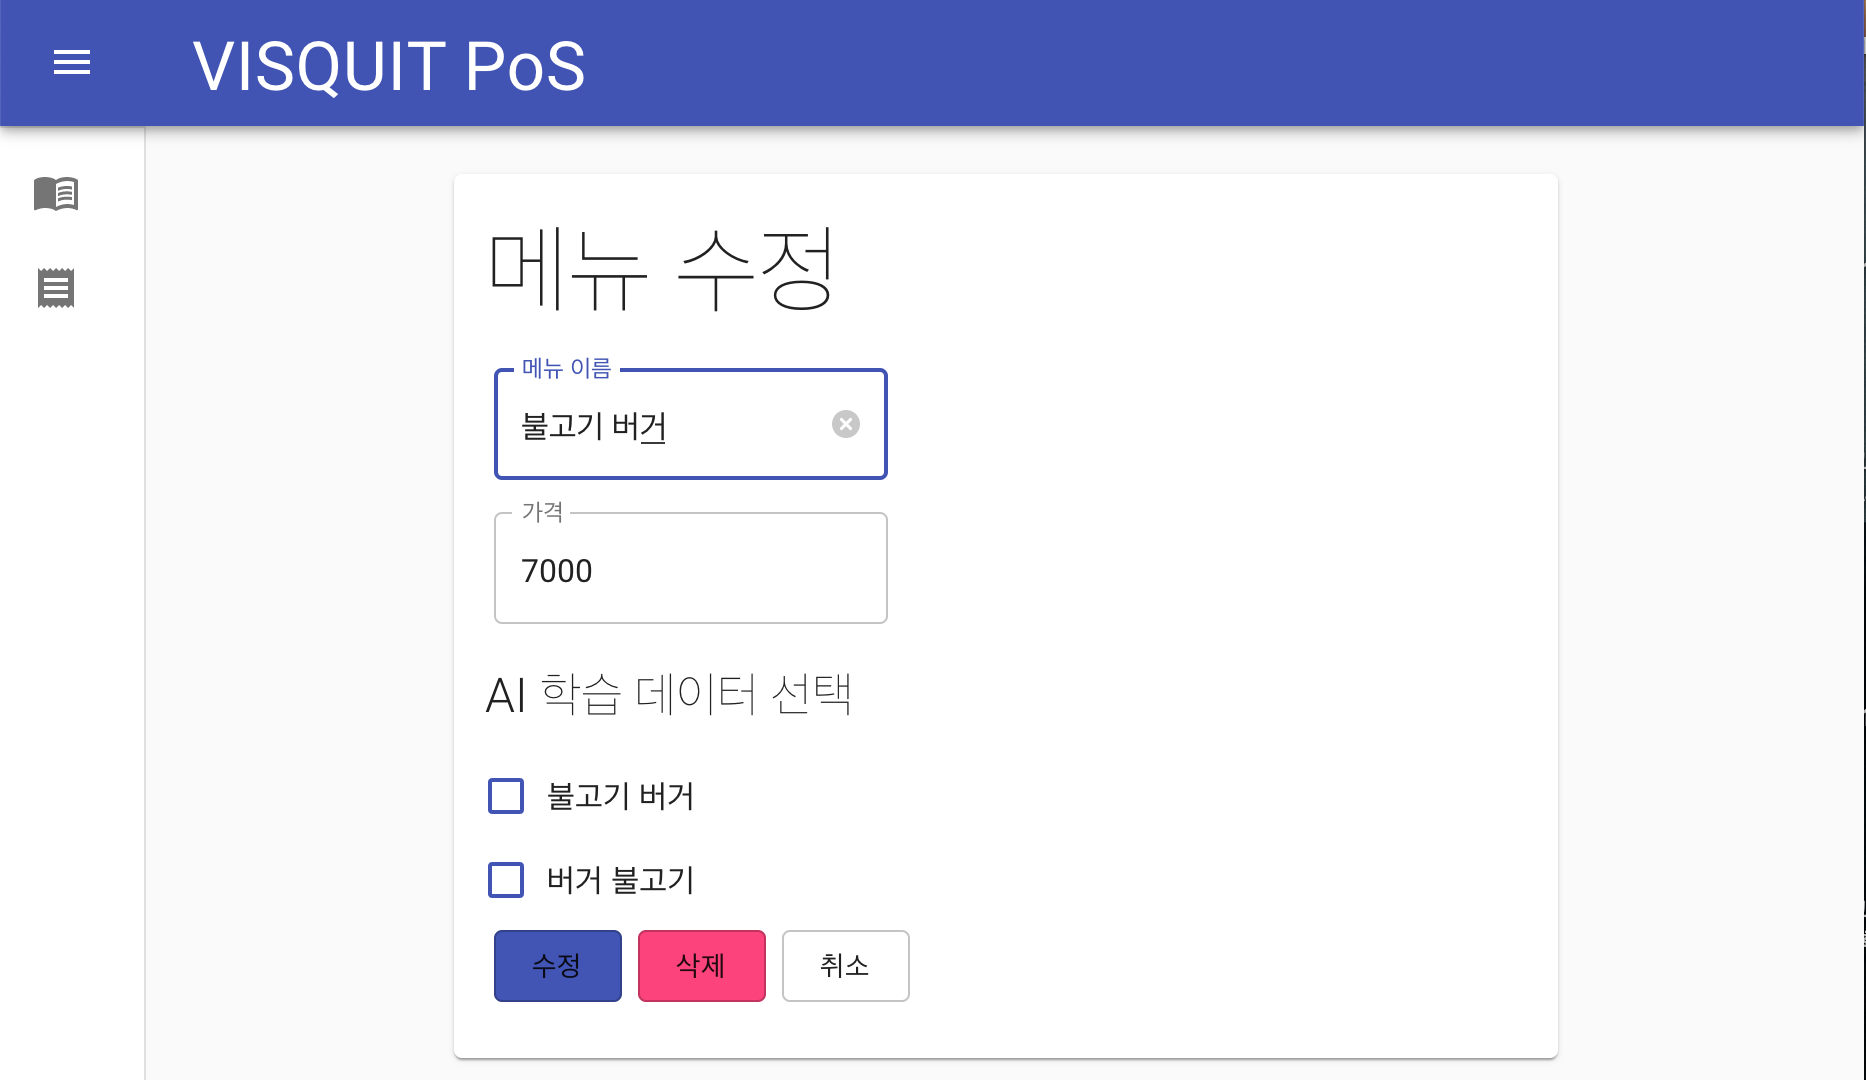
\includegraphics[width=\linewidth]{figures/frontend/06-editmenu-landing.png}
  \caption{Editting previous menu}
  \label{fig:06-editmenu-landing}
\end{figure}
\begin{figure}[ht!]
  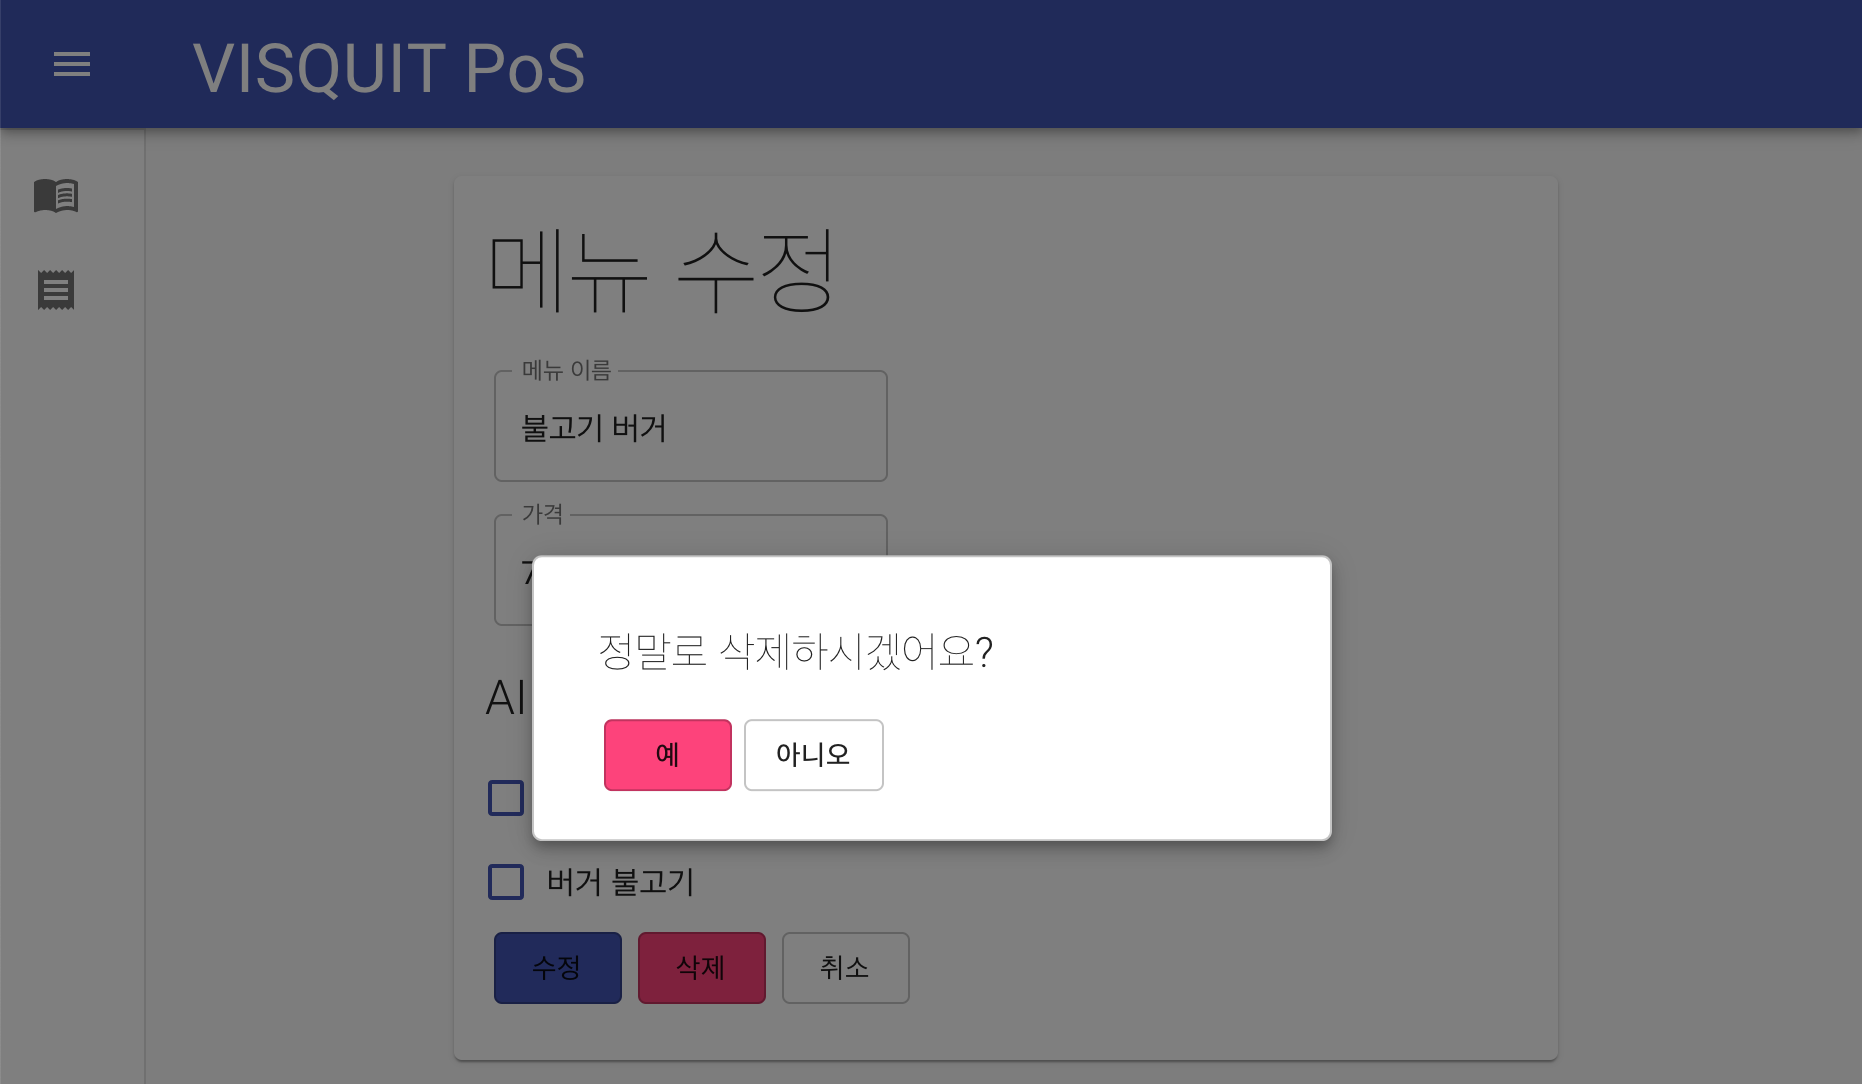
\includegraphics[width=\linewidth]{figures/frontend/07-editmenu-modal.png}
  \caption{Prompting Modal for each actions}
  \label{fig:07-editmenu-modal}
\end{figure}

When clicking a item on the '메뉴 목록' page, the user will be routed to 'Edit Menu' page. The features provided is identitcal to 'Add New Menu', except the target menu already exists. A modal will appear when an action is triggered as well.

\subsubsection{View Current Order List}

\begin{figure}[ht!]
  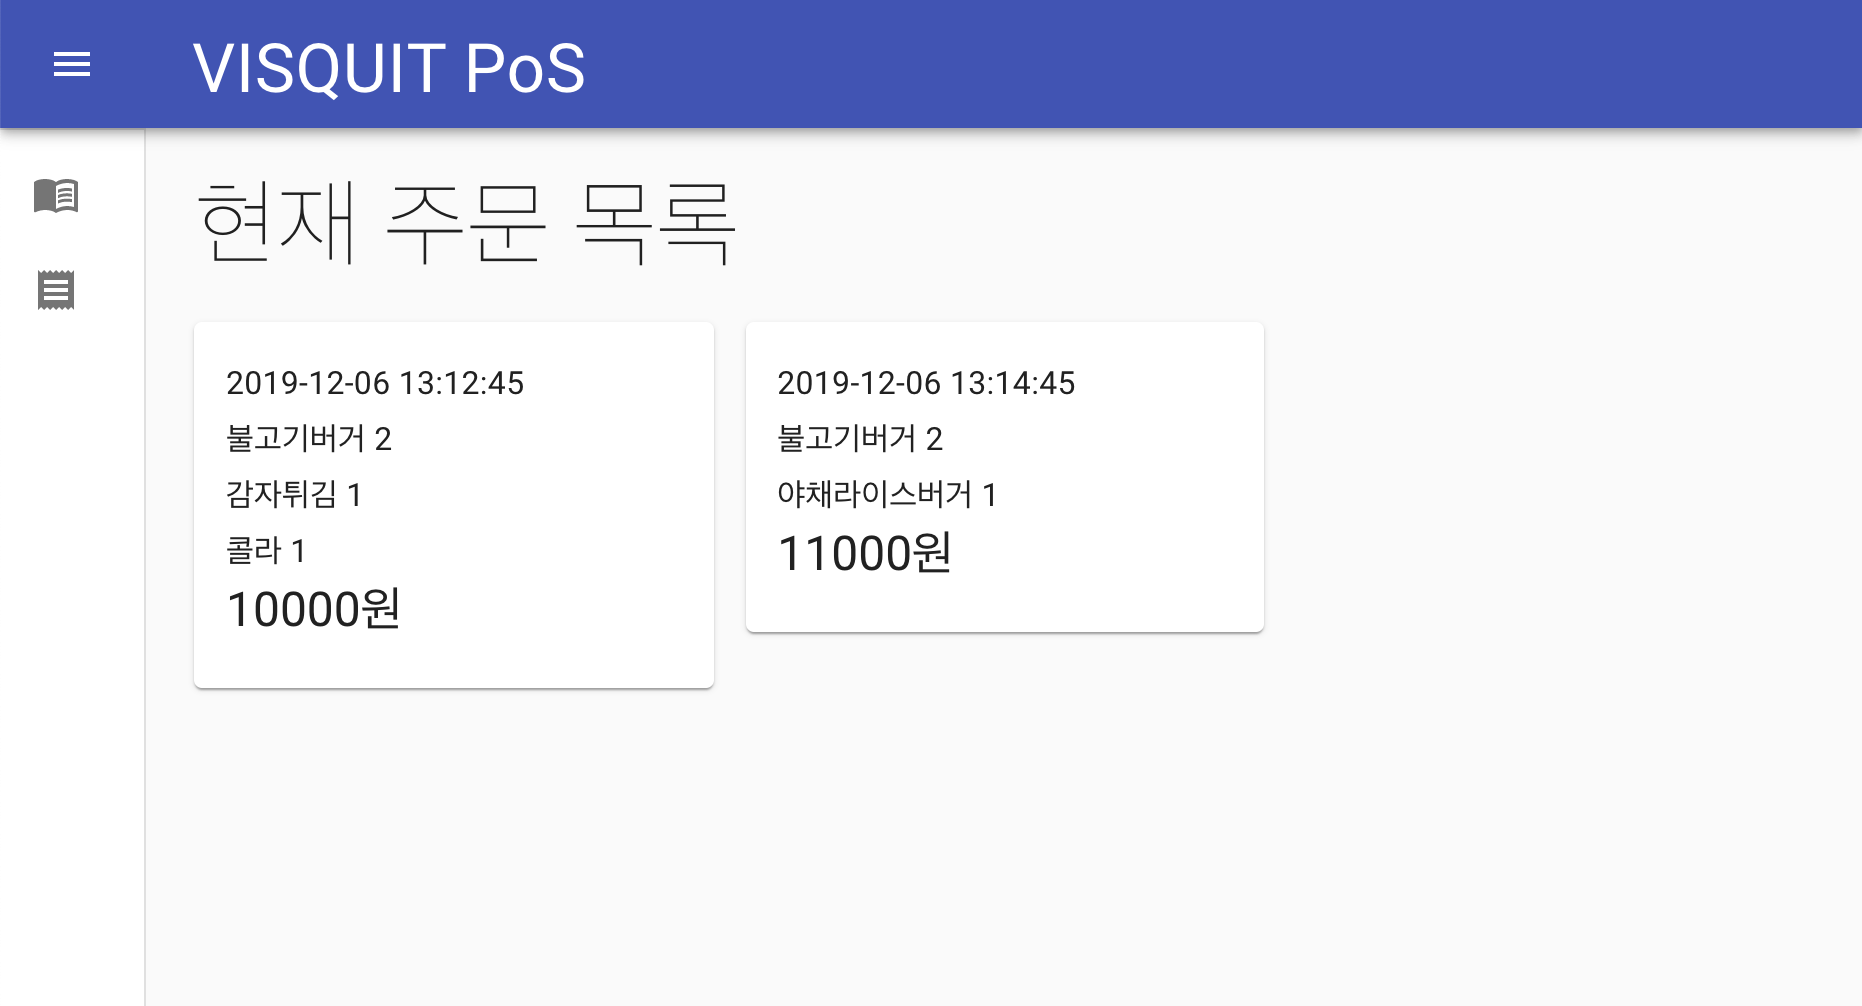
\includegraphics[width=\linewidth]{figures/frontend/08-orderlist.png}
  \caption{View Current Order List}
  \label{fig:08-orderlist}
\end{figure}

When clicking '현재 주문 목록' button on the left-side menu, the user will be routed to the page where the user can view all orders pending. 

\subsubsection{Process Pending Orders}

\begin{figure}[ht!]
  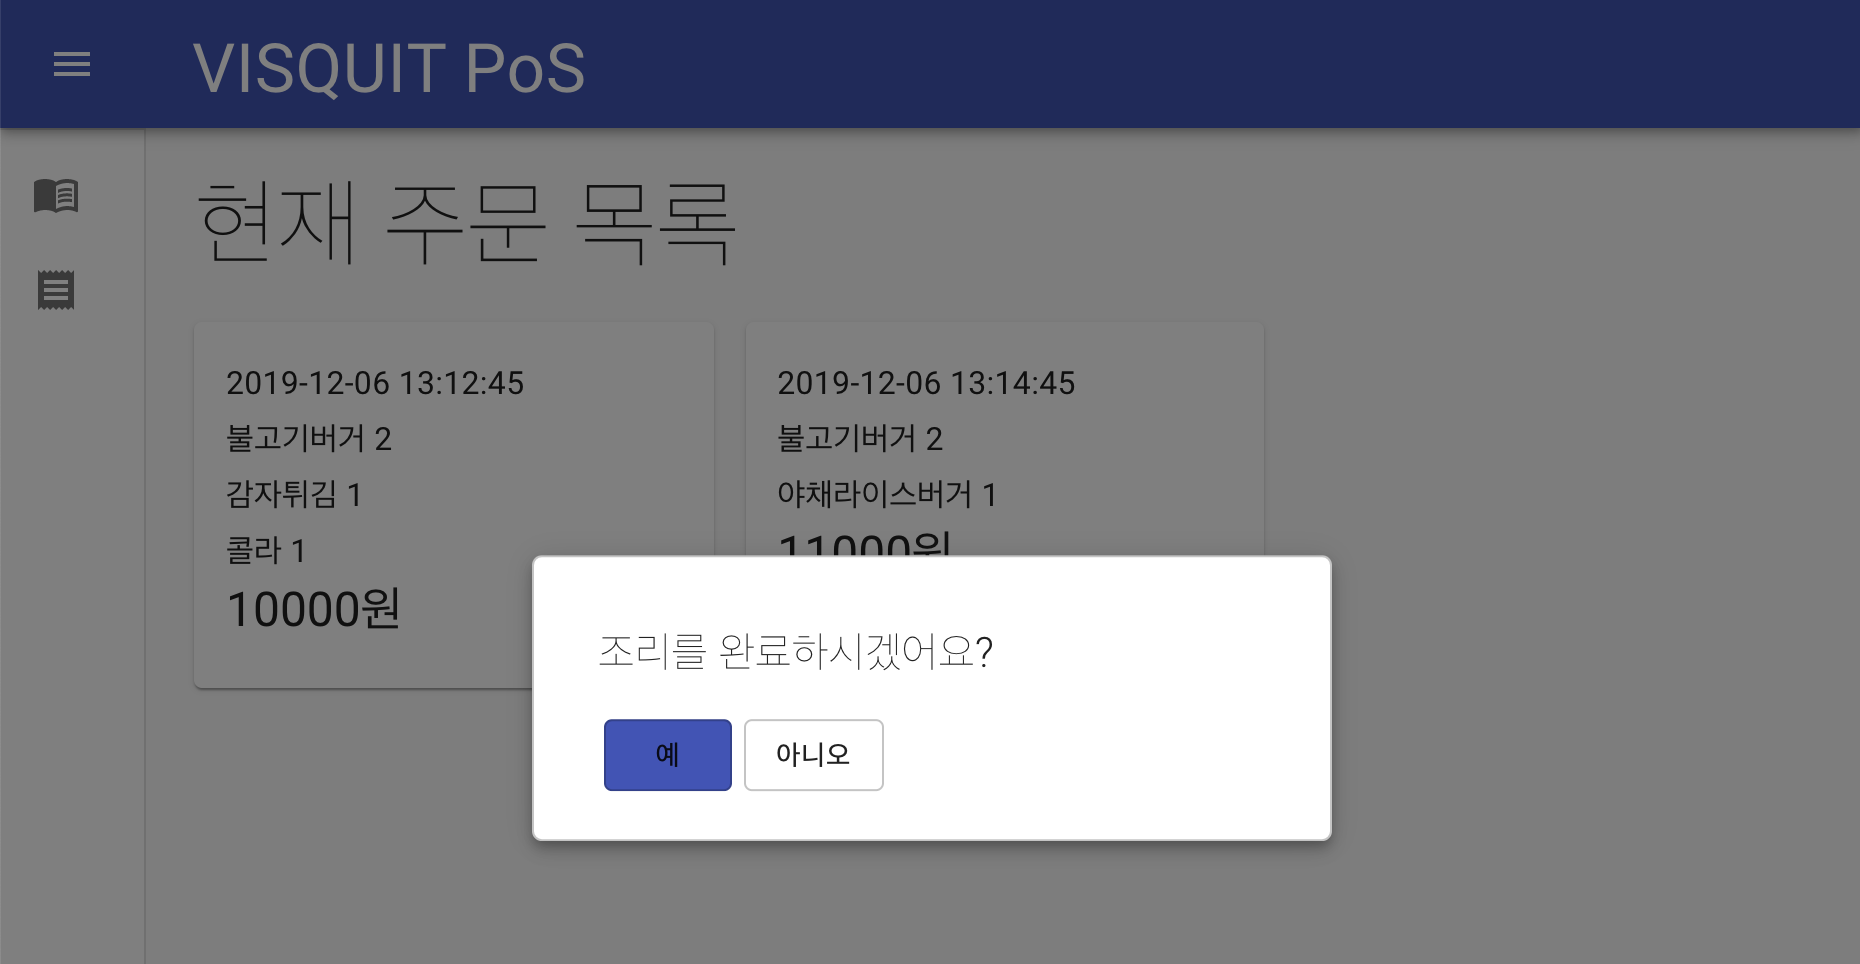
\includegraphics[width=\linewidth]{figures/frontend/09-order-finish-modal.png}
  \caption{View Current Order List}
  \label{fig:09-order-finish-modal}
\end{figure}

When clicking a item on the '현재 주문 목록' page, the frontend UI will double-check whether the particular order is really done. When the user click '예', the order's status for ready will be changed to 'true'.

\section{Conclusion}
Our project started from a little thought of what kinds of discomfort would the digital illiterate experience. There are many kinds of problems the digital illituerate would suffer from, but the discomfort arisen relevant to meal would be a major problem because food is an important matter for any kind of human being. We hope the user experience for the digital illiterate ordering meals in a restaurant could be improved through our software.

While developing this project, each teammates are responsible for each components of the project respectively. Our project was able to be completed successfully by each teammates' hard work and strong sense of responsibility, as well as their outstanding skills. The software development managing methodologies we learnt during the class will be very helpful when we become software engineers in the near future.

% An example of a floating figure using the graphicx package.
% Note that \label must occur AFTER (or within) \caption.
% For figures, \caption should occur after the \includegraphics.
% Note that IEEEtran v1.7 and later has special internal code that
% is designed to preserve the operation of \label within \caption
% even when the captionsoff option is in effect. However, because
% of issues like this, it may be the safest practice to put all your
% \label just after \caption rather than within \caption{}.
%
% Reminder: the "draftcls" or "draftclsnofoot", not "draft", class
% option should be used if it is desired that the figures are to be
% displayed while in draft mode.
%
%\begin{figure}[!t]
%\centering
%\includegraphics[width=2.5in]{myfigure}
% where an .eps filename suffix will be assumed under latex,
% and a .pdf suffix will be assumed for pdflatex; or what has been declared
% via \DeclareGraphicsExtensions.
%\caption{Simulation results for the network.}
%\label{fig_sim}
%\end{figure}

% Note that the IEEE typically puts floats only at the top, even when this
% results in a large percentage of a column being occupied by floats.


% An example of a double column floating figure using two subfigures.
% (The subfig.sty package must be loaded for this to work.)
% The subfigure \label commands are set within each subfloat command,
% and the \label for the overall figure must come after \caption.
% \hfil is used as a separator to get equal spacing.
% Watch out that the combined width of all the subfigures on a
% line do not exceed the text width or a line break will occur.
%
%\begin{figure*}[!t]
%\centering
%\subfloat[Case I]{\includegraphics[width=2.5in]{box}%
%\label{fig_first_case}}
%\hfil
%\subfloat[Case II]{\includegraphics[width=2.5in]{box}%
%\label{fig_second_case}}
%\caption{Simulation results for the network.}
%\label{fig_sim}
%\end{figure*}
%
% Note that often IEEE papers with subfigures do not employ subfigure
% captions (using the optional argument to \subfloat[]), but instead will
% reference/describe all of them (a), (b), etc., within the main caption.
% Be aware that for subfig.sty to generate the (a), (b), etc., subfigure
% labels, the optional argument to \subfloat must be present. If a
% subcaption is not desired, just leave its contents blank,
% e.g., \subfloat[].


% An example of a floating table. Note that, for IEEE style tables, the
% \caption command should come BEFORE the table and, given that table
% captions serve much like titles, are usually capitalized except for words
% such as a, an, and, as, at, but, by, for, in, nor, of, on, or, the, to
% and up, which are usually not capitalized unless they are the first or
% last word of the caption. Table text will default to \footnotesize as
% the IEEE normally uses this smaller font for tables.
% The \label must come after \caption as always.
%
%\begin{table}[!t]
%% increase table row spacing, adjust to taste
%\renewcommand{\arraystretch}{1.3}
% if using array.sty, it might be a good idea to tweak the value of
% \extrarowheight as needed to properly center the text within the cells
%\caption{An Example of a Table}
%\label{table_example}
%\centering
%% Some packages, such as MDW tools, offer better commands for making tables
%% than the plain LaTeX2e tabular which is used here.
%\begin{tabular}{|c||c|}
%\hline
%One & Two\\
%\hline
%Three & Four\\
%\hline
%\end{tabular}
%\end{table}


% Note that the IEEE does not put floats in the very first column
% - or typically anywhere on the first page for that matter. Also,
% in-text middle ("here") positioning is typically not used, but it
% is allowed and encouraged for Computer Society conferences (but
% not Computer Society journals). Most IEEE journals/conferences use
% top floats exclusively.
% Note that, LaTeX2e, unlike IEEE journals/conferences, places
% footnotes above bottom floats. This can be corrected via the
% \fnbelowfloat command of the stfloats package.


% conference papers do not normally have an appendix

% use section* for acknowledgment
% \ifCLASSOPTIONcompsoc
%   % The Computer Society usually uses the plural form
%   \section*{Acknowledgments}
% \else
%   % regular IEEE prefers the singular form
%   \section*{Acknowledgment}
% \fi

% trigger a \newpage just before the given reference
% number - used to balance the columns on the last page
% adjust value as needed - may need to be readjusted if
% the document is modified later
%\IEEEtriggeratref{8}
% The "triggered" command can be changed if desired:
%\IEEEtriggercmd{\enlargethispage{-5in}}

% references section

% can use a bibliography generated by BibTeX as a .bbl file
% BibTeX documentation can be easily obtained at:
% http://mirror.ctan.org/biblio/bibtex/contrib/doc/
% The IEEEtran BibTeX style support page is at:
% http://www.michaelshell.org/tex/ieeetran/bibtex/
%\bibliographystyle{IEEEtran}
% argument is your BibTeX string definitions and bibliography database(s)
%\bibliography{IEEEabrv,../bib/paper}
%
% <OR> manually copy in the resultant .bbl file
% set second argument of \begin to the number of references
% (used to reserve space for the reference number labels box)
% \begin{thebibliography}{1}

% \bibitem{IEEEhowto:kopka}
% H.~Kopka and P.~W. Daly, \emph{A Guide to \LaTeX}, 3rd~ed.\hskip 1em plus
%   0.5em minus 0.4em\relax Harlow, England: Addison-Wesley, 1999.

% \end{thebibliography}




% that's all folks
\end{document}
